% =============================================================================
% Appendix
% =============================================================================
% Note: graphicspath is inherited from main.tex; do NOT override it here.
% Numbering is handled by \appendix in main.tex (sections render as A, B, etc.)

% =============================================================================
\section{Additional Empirical Results}
\label{sec:app_empirical}

% --------------------------------------------------------------------------
\subsection{Representative Per-Asset Results}
\label{sec:app_per_asset}

One representative instrument from each asset class---BTC/USDT (cryptocurrency), EUR/USD (forex),
and Dow Jones/USA30IDXUSD (equity indices)---is presented below.  These are the HPO representative
assets and therefore provide the most controlled inter-model comparison.  \rmse bar charts for all
remaining instruments (ETH/USDT, BNB/USDT, ADA/USDT, USD/JPY, GBP/USD, AUD/USD, S\&P~500,
NASDAQ~100, and DAX), together with corresponding \mae and rank variants, are available in the Online
Supplementary Materials.  Results are reported as mean~$\pm$~standard deviation across seeds 123,
456, and 789.

\subsubsection{Cryptocurrency}
\label{sec:app_crypto}

\begin{figure}[htbp]
  \centering
  
\includegraphics[width=0.45\textwidth]{figures/appendix/crypto/BTCUSDT/4/rmse_comparison_barplot_no_lstm.pdf}
  \hfill
  
\includegraphics[width=0.45\textwidth]{figures/appendix/crypto/BTCUSDT/24/rmse_comparison_barplot_no_lstm.pdf}
  \caption{\rmse comparison for BTC/USDT at $\hfour$ (left) and $\htwentyfour$ (right), excluding \lstm
           for visual clarity.  \patchtst and \moderntcn achieve the two lowest errors at $\hfour$;
           \moderntcn leads marginally at $\htwentyfour$.  Mean~$\pm$~std across three seeds.}
  \label{fig:btcusdt_rmse_h4_h24}
\end{figure}

\subsubsection{Forex}
\label{sec:app_forex}

\begin{figure}[htbp]
  \centering
  
\includegraphics[width=0.45\textwidth]{figures/appendix/forex/EURUSD/4/rmse_comparison_barplot_no_lstm.pdf}
  \hfill
  
\includegraphics[width=0.45\textwidth]{figures/appendix/forex/EURUSD/24/rmse_comparison_barplot_no_lstm.pdf}
  \caption{\rmse comparison for EUR/USD at $\hfour$ (left) and $\htwentyfour$ (right), excluding \lstm.
           \moderntcn and \patchtst rank highest across both horizons; the remaining modern architectures
           cluster within a narrow error band.  Mean~$\pm$~std across three seeds.}
  \label{fig:eurusd_rmse_h4_h24}
\end{figure}

\subsubsection{Equity Indices}
\label{sec:app_indices}

\begin{figure}[htbp]
  \centering
  
\includegraphics[width=0.45\textwidth]{figures/appendix/indices/USA30IDXUSD/4/rmse_comparison_barplot_no_lstm.pdf}
  \hfill
  
\includegraphics[width=0.45\textwidth]{figures/appendix/indices/USA30IDXUSD/24/rmse_comparison_barplot_no_lstm.pdf}
  \caption{\rmse comparison for Dow Jones (USA30IDXUSD) at $\hfour$ (left) and $\htwentyfour$ (right),
           excluding \lstm.  \moderntcn ranks first at both horizons; \patchtst follows closely.
           Mean~$\pm$~std across three seeds.}
  \label{fig:usa30idxusd_rmse_h4_h24}
\end{figure}

% --------------------------------------------------------------------------
\subsection{Remaining Per-Asset Results}
\label{sec:app_remaining_assets}

Figures~\ref{fig:ethusdt_rmse_h4_h24}--\ref{fig:usatechidxusd_rmse_h4_h24} present \rmse
bar charts for the nine assets not shown in Section~\ref{sec:app_per_asset}, completing the
full 12-asset comparison.  Across all assets, the three-tier structure
(\moderntcn/\patchtst at top; \itransformer/\timexer/\dlinear/\nhits in the middle;
\timesnet/\autoformer at the bottom) is maintained, with the notable exception of
ETH/USDT and ADA/USDT where \nhits achieves the lowest \rmse
(Table~\ref{tab:per_asset_best_models}).

\subsubsection{Cryptocurrency --- Remaining Assets}

\begin{figure}[htbp]
  \centering
  
\includegraphics[width=0.45\textwidth]{figures/appendix/crypto/ETHUSDT/4/rmse_comparison_barplot_no_lstm.pdf}
  \hfill
  
\includegraphics[width=0.45\textwidth]{figures/appendix/crypto/ETHUSDT/24/rmse_comparison_barplot_no_lstm.pdf}
  \caption{\rmse comparison for ETH/USDT at $\hfour$ (left) and $\htwentyfour$ (right),
           excluding \lstm.  \nhits achieves the lowest \rmse at both horizons,
           one of only two assets where \moderntcn does not rank first.
           Mean~$\pm$~std across three seeds.}
  \label{fig:ethusdt_rmse_h4_h24}
\end{figure}

\begin{figure}[htbp]
  \centering
  
\includegraphics[width=0.45\textwidth]{figures/appendix/crypto/BNBUSDT/4/rmse_comparison_barplot_no_lstm.pdf}
  \hfill
  
\includegraphics[width=0.45\textwidth]{figures/appendix/crypto/BNBUSDT/24/rmse_comparison_barplot_no_lstm.pdf}
  \caption{\rmse comparison for BNB/USDT at $\hfour$ (left) and $\htwentyfour$ (right),
           excluding \lstm.  \moderntcn leads at both horizons with a clear margin.
           Mean~$\pm$~std across three seeds.}
  \label{fig:bnbusdt_rmse_h4_h24}
\end{figure}

\begin{figure}[htbp]
  \centering
  
\includegraphics[width=0.45\textwidth]{figures/appendix/crypto/ADAUSDT/4/rmse_comparison_barplot_no_lstm.pdf}
  \hfill
  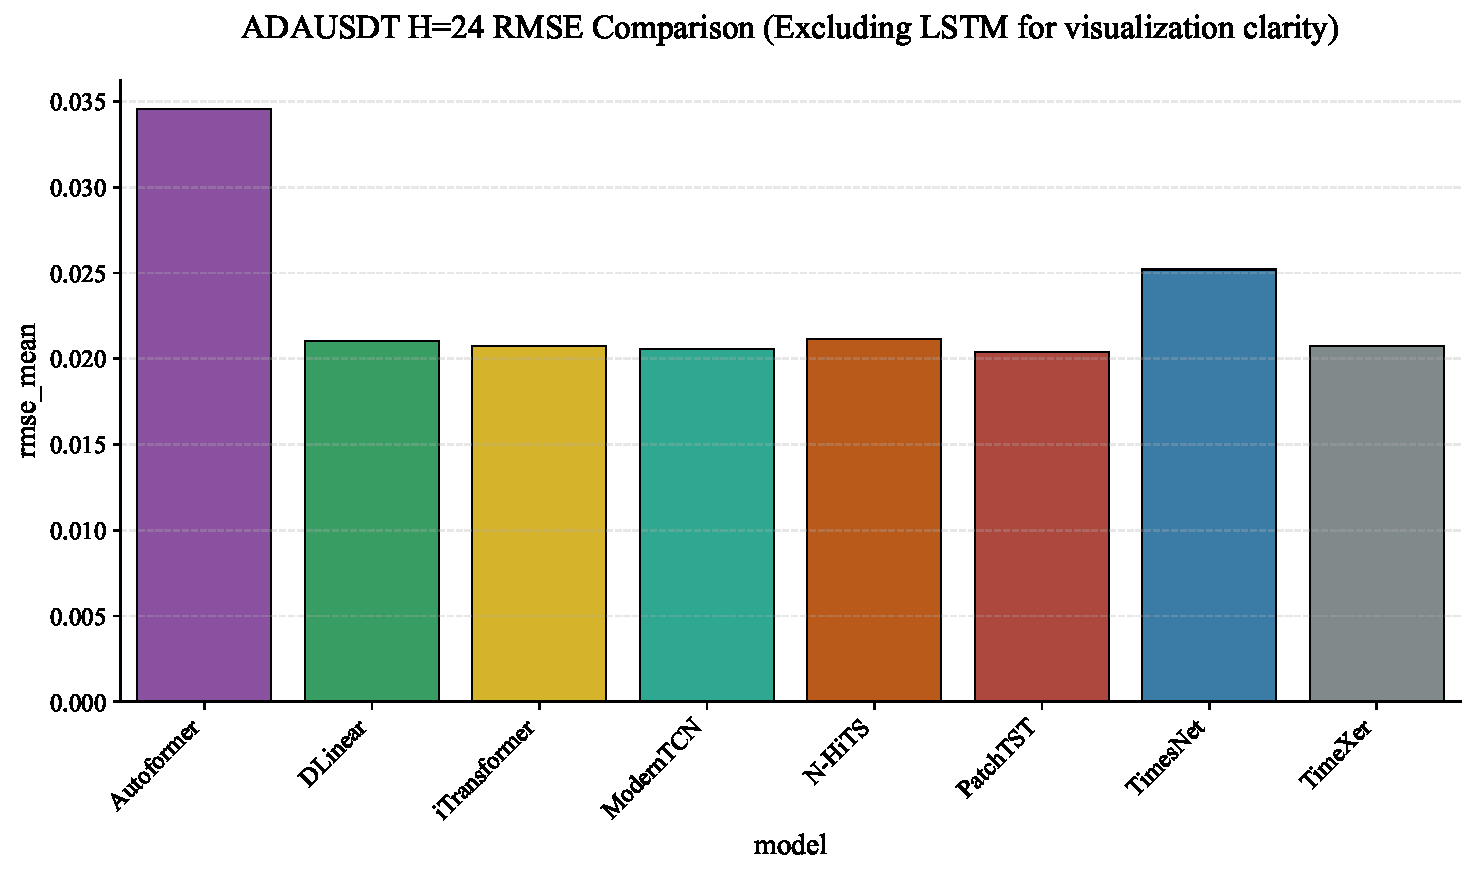
\includegraphics[width=0.45\textwidth]{figures/appendix/crypto/ADAUSDT/24/rmse_comparison_barplot_no_lstm.pdf}
  \caption{\rmse comparison for ADA/USDT at $\hfour$ (left) and $\htwentyfour$ (right),
           excluding \lstm.  \nhits leads at $\hfour$; \patchtst leads at $\htwentyfour$.
           This asset exhibits the lowest cross-horizon Spearman $\rho$ ($0.683$;
           Table~\ref{tab:stat_tests_spearman}), consistent with more variable
           rankings between horizons.
           Mean~$\pm$~std across three seeds.}
  \label{fig:adausdt_rmse_h4_h24}
\end{figure}

\subsubsection{Forex --- Remaining Assets}

\begin{figure}[htbp]
  \centering
  
\includegraphics[width=0.45\textwidth]{figures/appendix/forex/USDJPY/4/rmse_comparison_barplot_no_lstm.pdf}
  \hfill
  
\includegraphics[width=0.45\textwidth]{figures/appendix/forex/USDJPY/24/rmse_comparison_barplot_no_lstm.pdf}
  \caption{\rmse comparison for USD/JPY at $\hfour$ (left) and $\htwentyfour$ (right),
           excluding \lstm.  \moderntcn ranks first; the modern architecture cluster
           is tightly packed.
           Mean~$\pm$~std across three seeds.}
  \label{fig:usdjpy_rmse_h4_h24}
\end{figure}

\begin{figure}[htbp]
  \centering
  
\includegraphics[width=0.45\textwidth]{figures/appendix/forex/GBPUSD/4/rmse_comparison_barplot_no_lstm.pdf}
  \hfill
  
\includegraphics[width=0.45\textwidth]{figures/appendix/forex/GBPUSD/24/rmse_comparison_barplot_no_lstm.pdf}
  \caption{\rmse comparison for GBP/USD at $\hfour$ (left) and $\htwentyfour$ (right),
           excluding \lstm.  \patchtst leads at $\hfour$; \moderntcn leads
           at $\htwentyfour$.  Mean~$\pm$~std across three seeds.}
  \label{fig:gbpusd_rmse_h4_h24}
\end{figure}

\begin{figure}[htbp]
  \centering
  
\includegraphics[width=0.45\textwidth]{figures/appendix/forex/AUDUSD/4/rmse_comparison_barplot_no_lstm.pdf}
  \hfill
  
\includegraphics[width=0.45\textwidth]{figures/appendix/forex/AUDUSD/24/rmse_comparison_barplot_no_lstm.pdf}
  \caption{\rmse comparison for AUD/USD at $\hfour$ (left) and $\htwentyfour$ (right),
           excluding \lstm.  \moderntcn ranks first at both horizons.
           Mean~$\pm$~std across three seeds.}
  \label{fig:audusd_rmse_h4_h24}
\end{figure}

\subsubsection{Equity Indices --- Remaining Assets}

\begin{figure}[htbp]
  \centering
  
\includegraphics[width=0.45\textwidth]{figures/appendix/indices/DEUIDXEUR/4/rmse_comparison_barplot_no_lstm.pdf}
  \hfill
  
\includegraphics[width=0.45\textwidth]{figures/appendix/indices/DEUIDXEUR/24/rmse_comparison_barplot_no_lstm.pdf}
  \caption{\rmse comparison for DAX (DEUIDXEUR) at $\hfour$ (left) and $\htwentyfour$ (right),
           excluding \lstm.  \moderntcn leads at both horizons; the top-four
           cluster (\moderntcn, \patchtst, \itransformer, \timexer) is tightly grouped.
           Mean~$\pm$~std across three seeds.}
  \label{fig:deuidxeur_rmse_h4_h24}
\end{figure}

\begin{figure}[htbp]
  \centering
  
\includegraphics[width=0.45\textwidth]{figures/appendix/indices/USA500IDXUSD/4/rmse_comparison_barplot_no_lstm.pdf}
  \hfill
  
\includegraphics[width=0.45\textwidth]{figures/appendix/indices/USA500IDXUSD/24/rmse_comparison_barplot_no_lstm.pdf}
  \caption{\rmse comparison for S\&P~500 (USA500IDXUSD) at $\hfour$ (left) and $\htwentyfour$ (right),
           excluding \lstm.  \moderntcn leads; the cross-horizon Spearman
           $\rho = 0.967$ (Table~\ref{tab:stat_tests_spearman}) indicates near-perfect
           rank preservation.  Mean~$\pm$~std across three seeds.}
  \label{fig:usa500idxusd_rmse_h4_h24}
\end{figure}

\begin{figure}[htbp]
  \centering
  
\includegraphics[width=0.45\textwidth]{figures/appendix/indices/USATECHIDXUSD/4/rmse_comparison_barplot_no_lstm.pdf}
  \hfill
  
\includegraphics[width=0.45\textwidth]{figures/appendix/indices/USATECHIDXUSD/24/rmse_comparison_barplot_no_lstm.pdf}
  \caption{\rmse comparison for NASDAQ~100 (USATECHIDXUSD) at $\hfour$ (left) and $\htwentyfour$ (right),
           excluding \lstm.  \moderntcn leads; the cross-horizon Spearman
           $\rho = 0.983$ (Table~\ref{tab:stat_tests_spearman}) is the highest
           among all assets.  Mean~$\pm$~std across three seeds.}
  \label{fig:usatechidxusd_rmse_h4_h24}
\end{figure}

% --------------------------------------------------------------------------
\subsection{Cross-Horizon Analysis}
\label{sec:app_horizon}

Figure~\ref{fig:app_horizon_degradation_all} reproduces the horizon-degradation line plot from the
main text (Figure~\ref{fig:horizon_degradation}) with all \nmodels models included.  The no-\lstm
variant is used as the primary reference because \lstm's elevated baseline
compresses the vertical scale, obscuring differences among the eight modern architectures.

\begin{figure}[htbp]
  \centering
  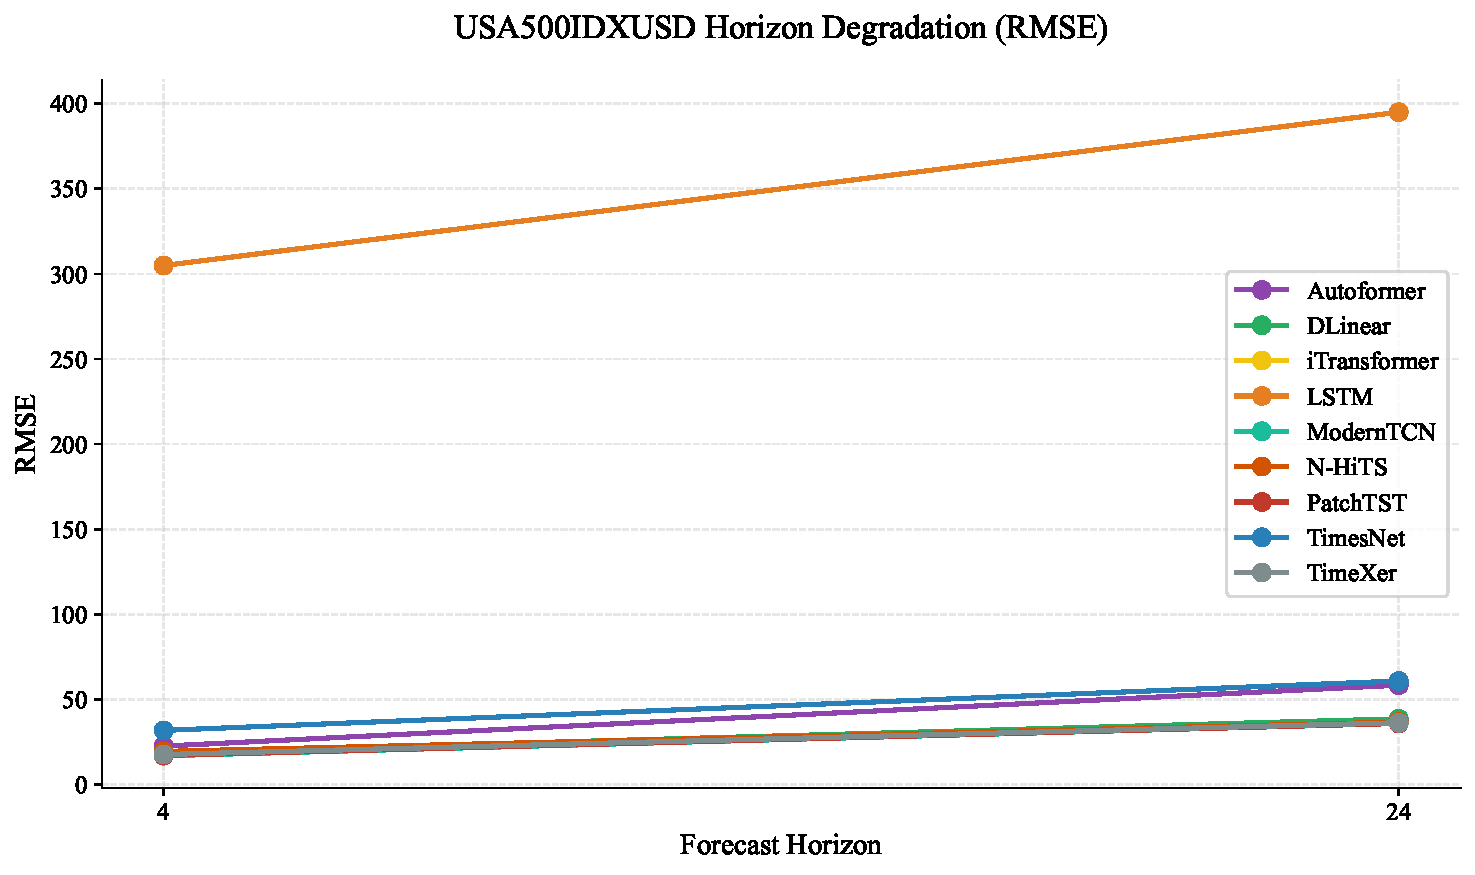
\includegraphics[width=0.75\textwidth]{figures/05_horizon_analysis/horizon_degradation_lineplot.pdf}
  \caption{Cross-horizon \rmse degradation for all \nmodels models.
           Compare with Figure~\ref{fig:horizon_degradation} (no-\lstm variant) for finer inter-model
           discrimination.}
  \label{fig:app_horizon_degradation_all}
\end{figure}

% --------------------------------------------------------------------------
\subsection{Horizon Sensitivity Heatmap}
\label{sec:app_horizon_sensitivity}

Figure~\ref{fig:app_horizon_sensitivity_heatmap} displays the percentage \rmse
degradation from $\hfour$ to $\htwentyfour$ for each model--asset combination (excluding \lstm).
Cool cells indicate architectures whose representations transfer well
across horizons; warm cells highlight combinations where temporal structure
deteriorates rapidly with forecast depth.

\begin{figure}[htbp]
  \centering
  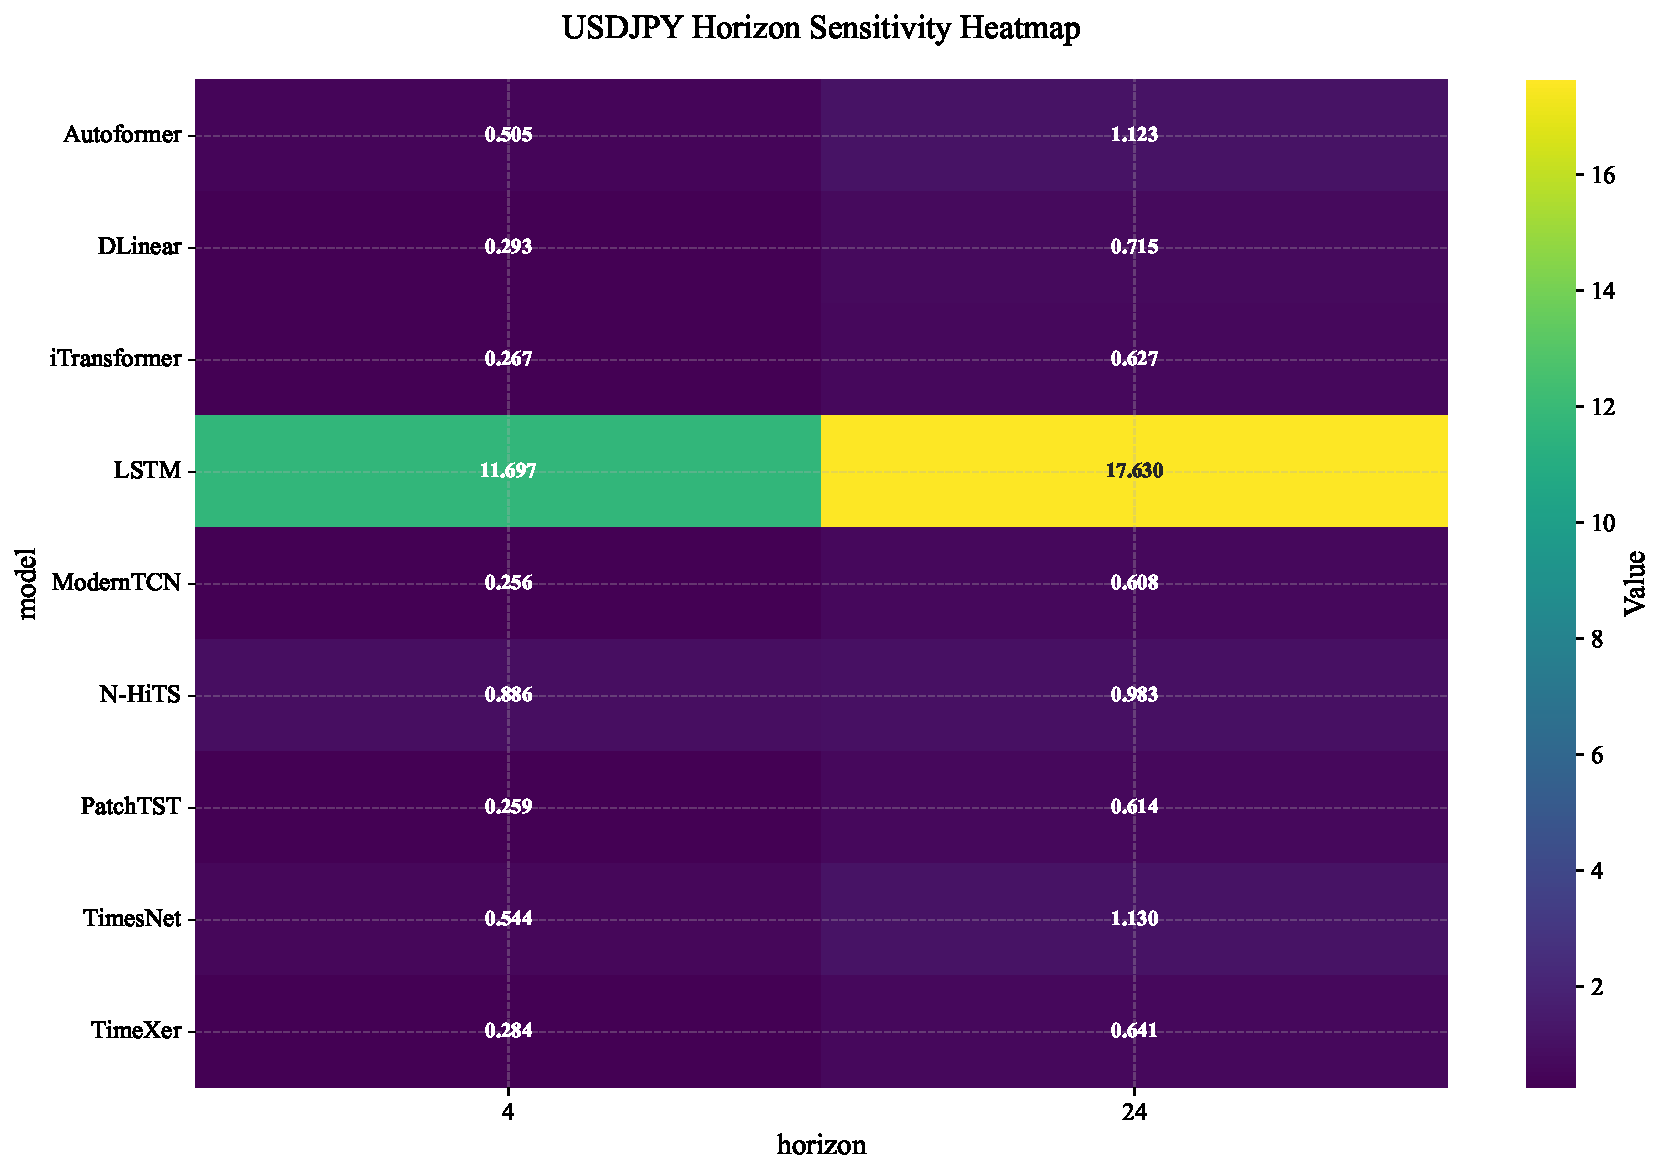
\includegraphics[width=0.85\textwidth]{figures/appendix/horizon_sensitivity_heatmap.pdf}
  \caption{Horizon sensitivity heatmap: percentage \rmse degradation
           ($\Delta\% = 100\times(\text{RMSE}_{24} - \text{RMSE}_4)/\text{RMSE}_4$)
           for eight modern architectures across all twelve assets.
           \lstm is excluded for visual clarity.
           Values below 90\% (low degradation) appear in cooler colours;
           values above 150\% appear in warmer shades.
           \nhits on Dow Jones achieves the lowest degradation (59.7\%);
           \timesnet on Dow Jones the highest (169.1\%).}
  \label{fig:app_horizon_sensitivity_heatmap}
\end{figure}

% --------------------------------------------------------------------------
\subsection{Dual-Plot Variants (All Models Including \lstm)}
\label{sec:app_dual_plots}

Figure~\ref{fig:app_global_heatmap_all} shows the global \rmse heatmap including all nine models; compare with Figure~\ref{fig:global_heatmap} for finer discrimination among modern architectures.  Figure~\ref{fig:app_asset_model_comparison_grouped_all} presents the cross-horizon comparison for the full nine-model set.  \lstm produces the highest errors across all assets and horizons, with its error floor exceeding even the lowest-performing modern architectures.

\begin{figure}[htbp]
  \centering
  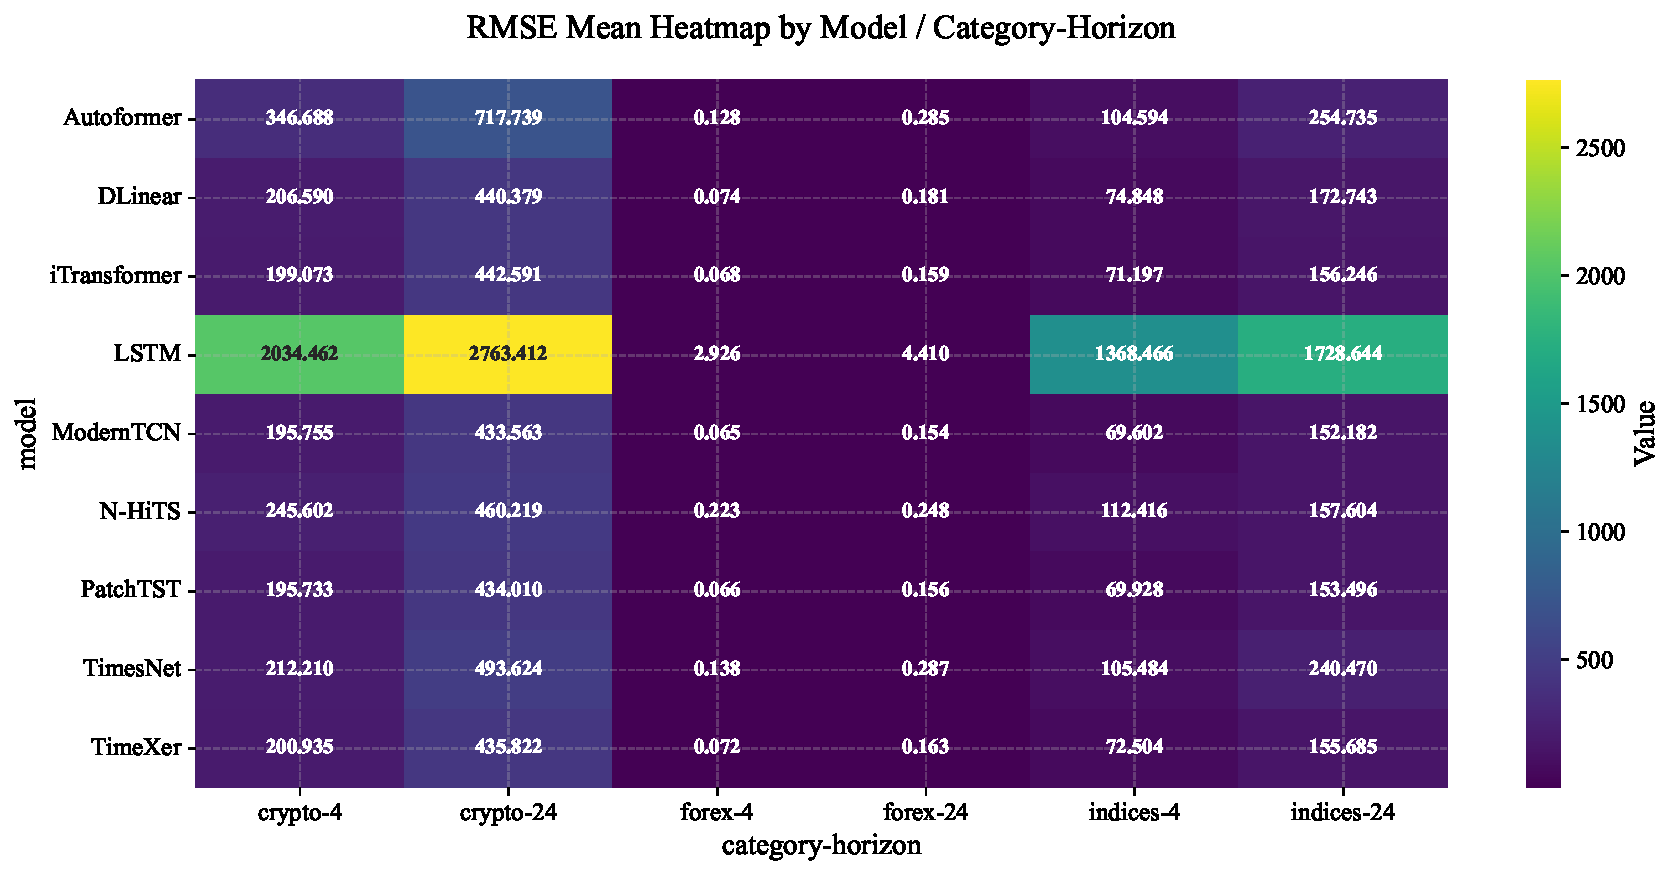
\includegraphics[width=0.85\textwidth]{figures/03_global_performance/global_metric_heatmap.pdf}
  \caption{Global \rmse heatmap for all \nmodels architectures (including \lstm) across 24 evaluation points.  \lstm's extreme errors dominate the colour scale, which is why the no-\lstm variant (Figure~\ref{fig:global_heatmap}) is used as the primary figure in the main body.}
  \label{fig:app_global_heatmap_all}
\end{figure}

\begin{figure}[htbp]
  \centering
  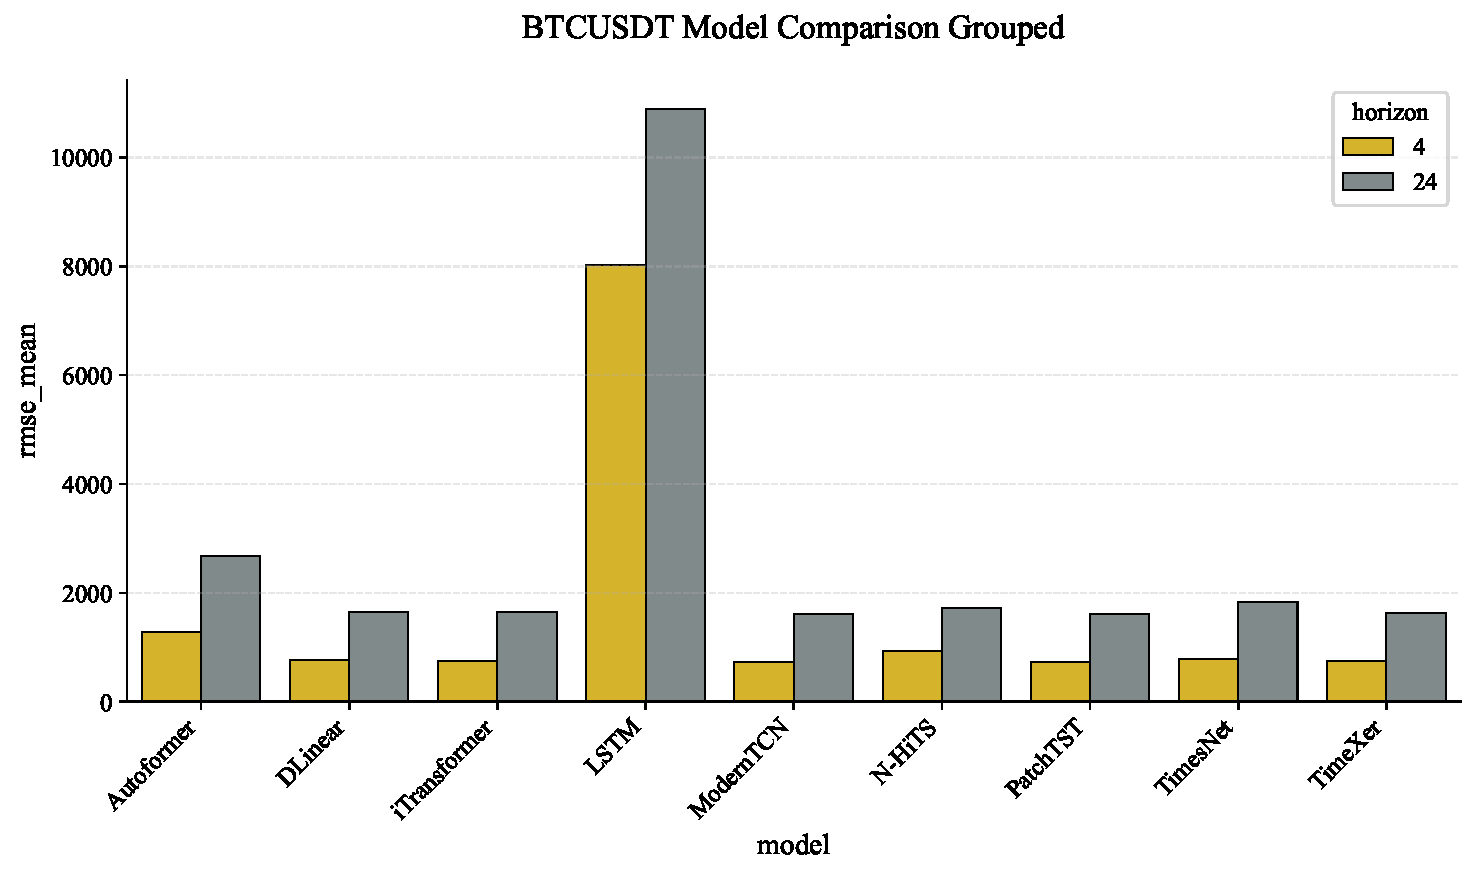
\includegraphics[width=\textwidth]{figures/04_category_analysis/asset_model_comparison_grouped.pdf}
  \caption{Cross-horizon \rmse comparison for all nine architectures across twelve assets, including \lstm.  The recurrent baseline illustrates the generational performance gap relative to modern time-series architectures.}
  \label{fig:app_asset_model_comparison_grouped_all}
\end{figure}

% --------------------------------------------------------------------------
\subsection{Appendix: Efficiency Including LSTM Models}
\label{sec:app_efficiency_lstm}

While the main-body analysis (Section~\ref{sec:complexity}) focuses on modern architectures, Figure~\ref{fig:app_complexity_full} includes \lstm.  Despite a parameter budget ($\approx 172{,}000$) that is moderate in absolute terms, \lstm achieves the worst ranking at both horizons, reinforcing that modern architectural components provide far higher return on parameter investment than recurrent inductive biases for this task.

\begin{figure}[htbp]
  \centering
  \begin{subfigure}[b]{0.48\textwidth}
    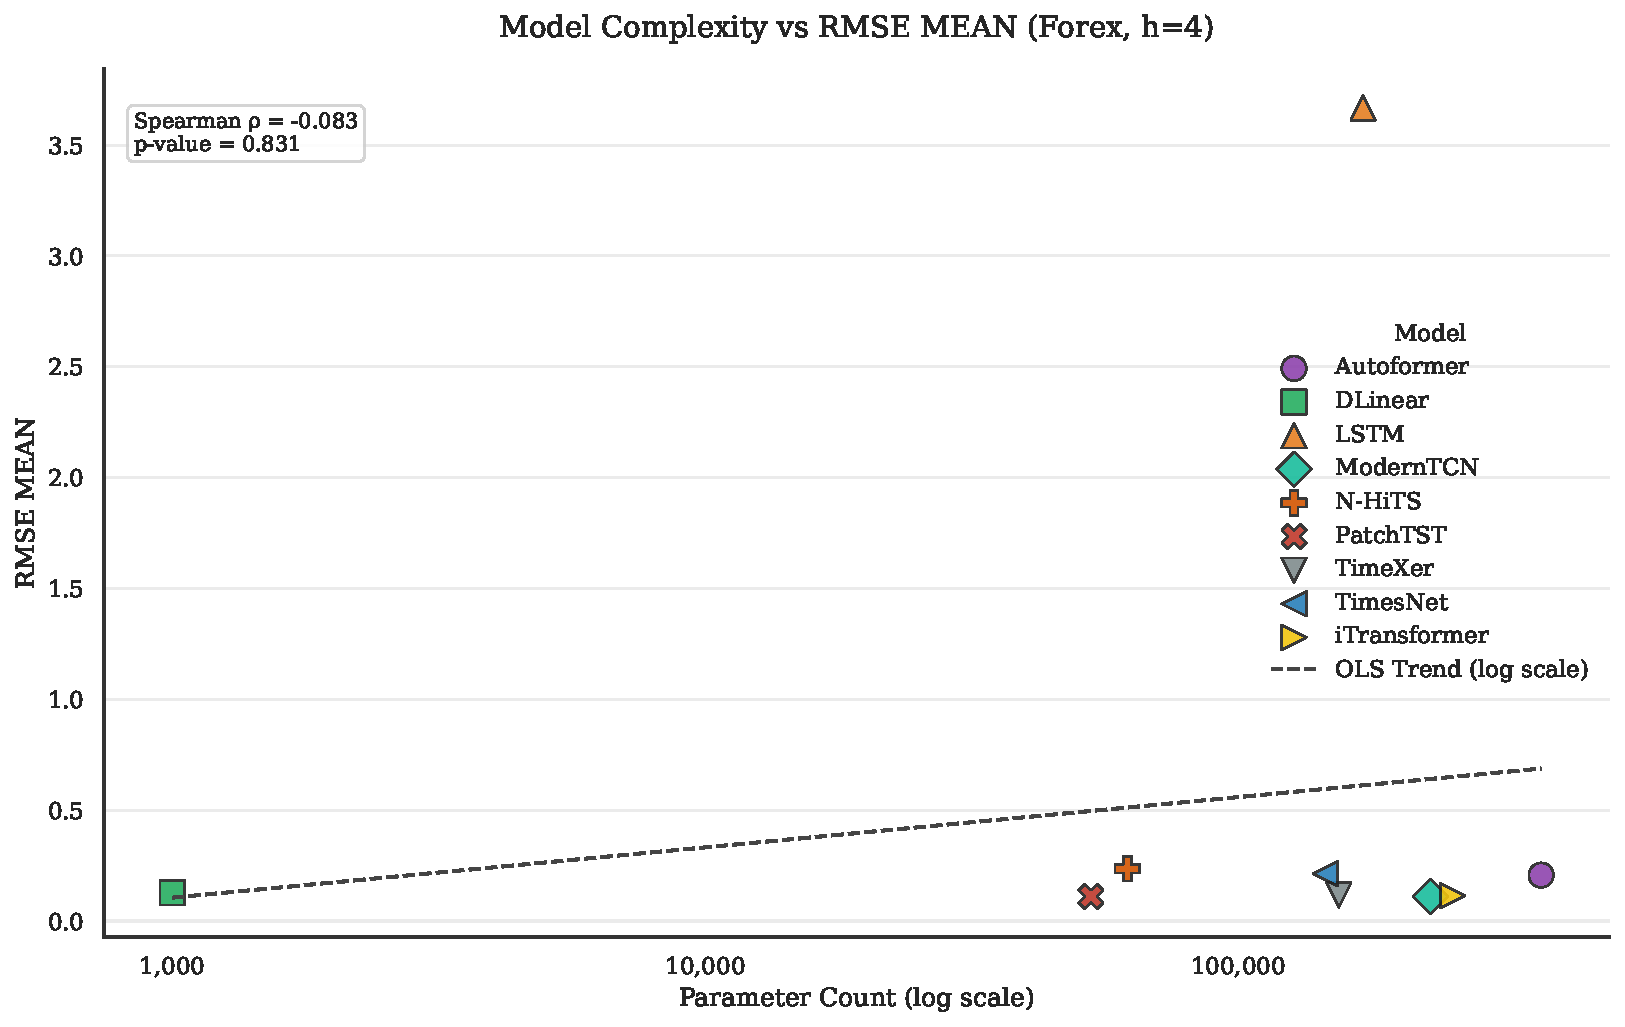
\includegraphics[width=\textwidth]{figures/07_efficiency/complexity_vs_performance_h4.pdf}
    \caption{Horizon $h=4$.}
    \label{fig:app_complexity_h4}
  \end{subfigure}
  \hfill
  \begin{subfigure}[b]{0.48\textwidth}
    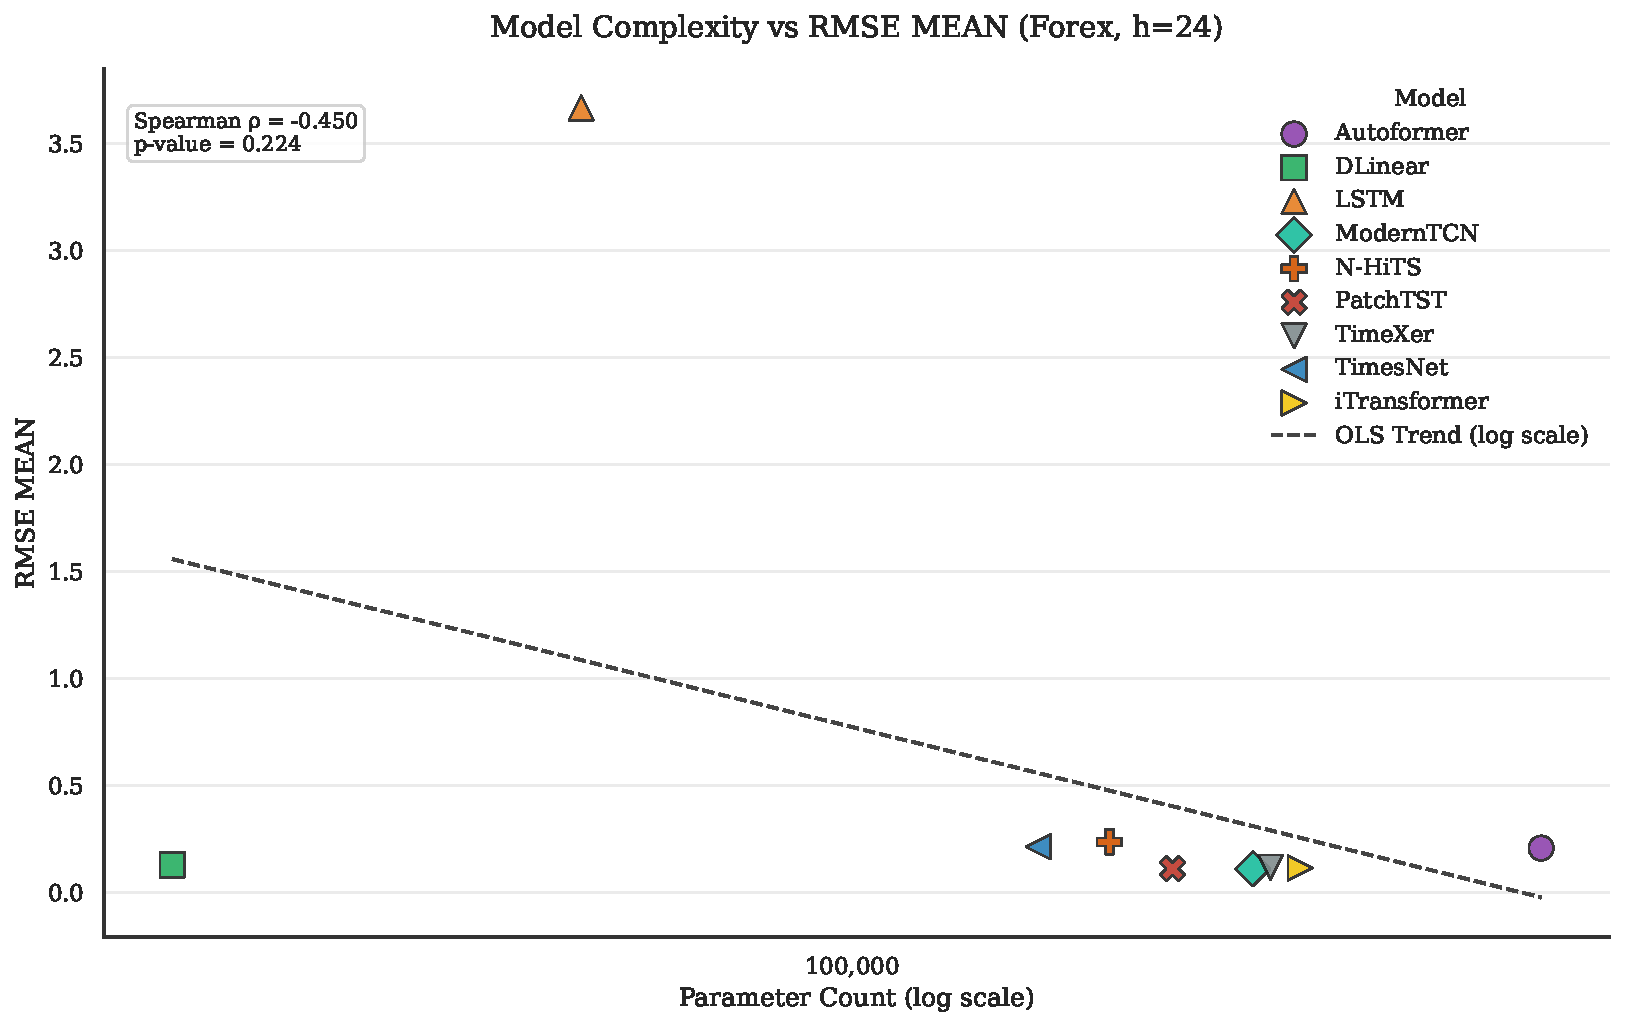
\includegraphics[width=\textwidth]{figures/07_efficiency/complexity_vs_performance_h24.pdf}
    \caption{Horizon $h=24$.}
    \label{fig:app_complexity_h24}
  \end{subfigure}
  \caption{Extended complexity--performance relationship including \lstm.  The recurrent baseline lies far from the Pareto frontier defined by modern architectures.}
  \label{fig:app_complexity_full}
\end{figure}

% --------------------------------------------------------------------------
\subsection{Category Hierarchical Rankings}
\label{sec:app_category_rankings}

Figures~\ref{fig:app_crypto_hier_ranking}--\ref{fig:app_indices_hier_ranking} display
hierarchical ranking dendrograms for each asset class, grouping architectures by
performance similarity.  These complement the leaderboard tables by revealing clustering
structure: closely branched architectures perform similarly; widely separated branches
indicate consistent performance gaps.  The no-\lstm variant is shown.

\begin{figure}[htbp]
  \centering
  \begin{subfigure}[b]{0.48\textwidth}
    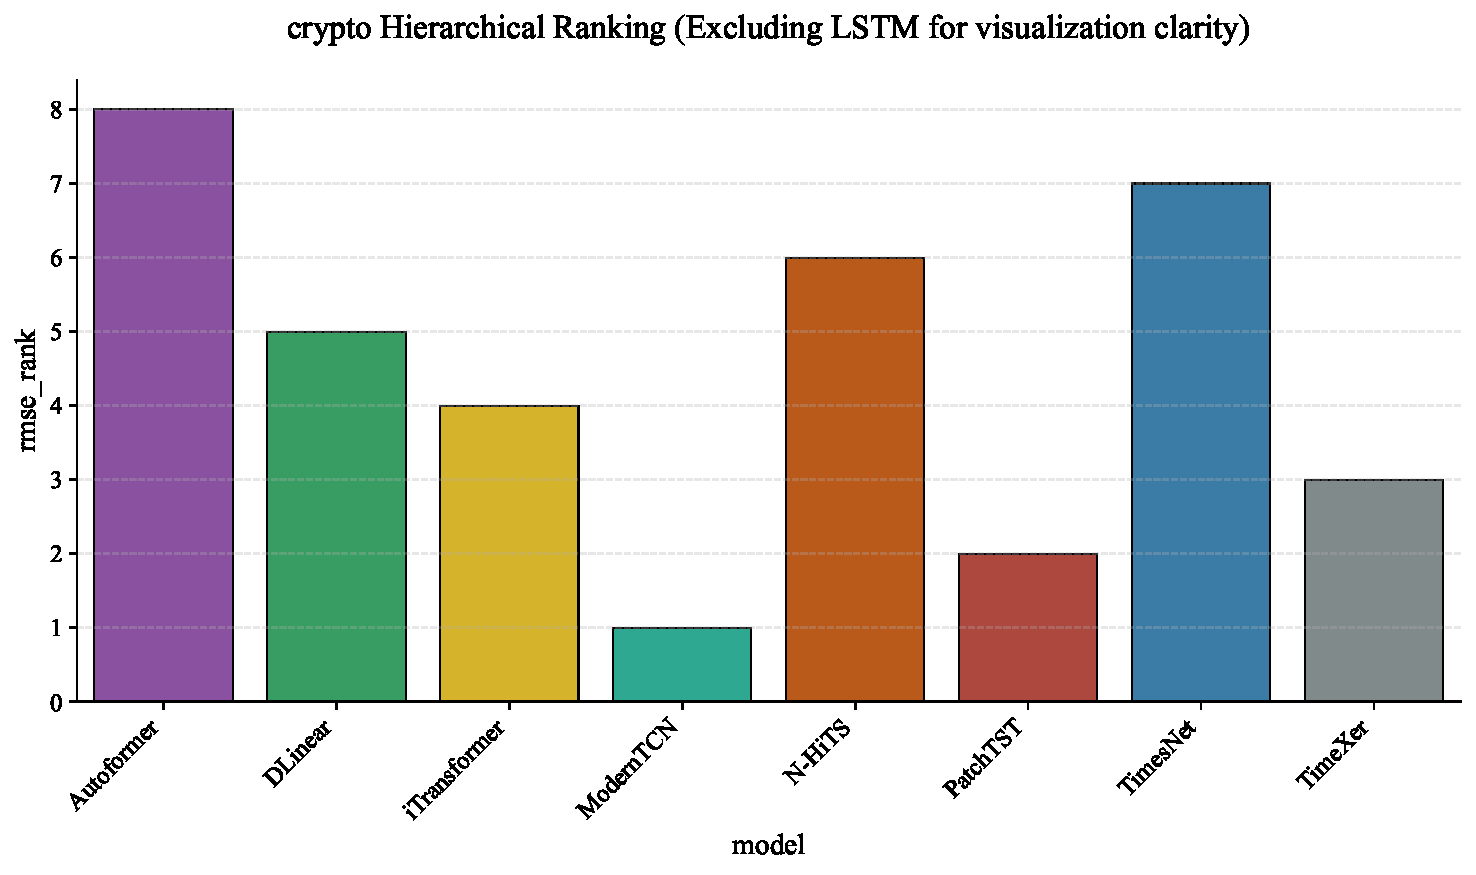
\includegraphics[width=\textwidth]{figures/04_category_analysis/crypto_category_hierarchical_ranking_no_lstm.pdf}
    \caption{Cryptocurrency.}
    \label{fig:app_crypto_hier_ranking}
  \end{subfigure}
  \hfill
  \begin{subfigure}[b]{0.48\textwidth}
    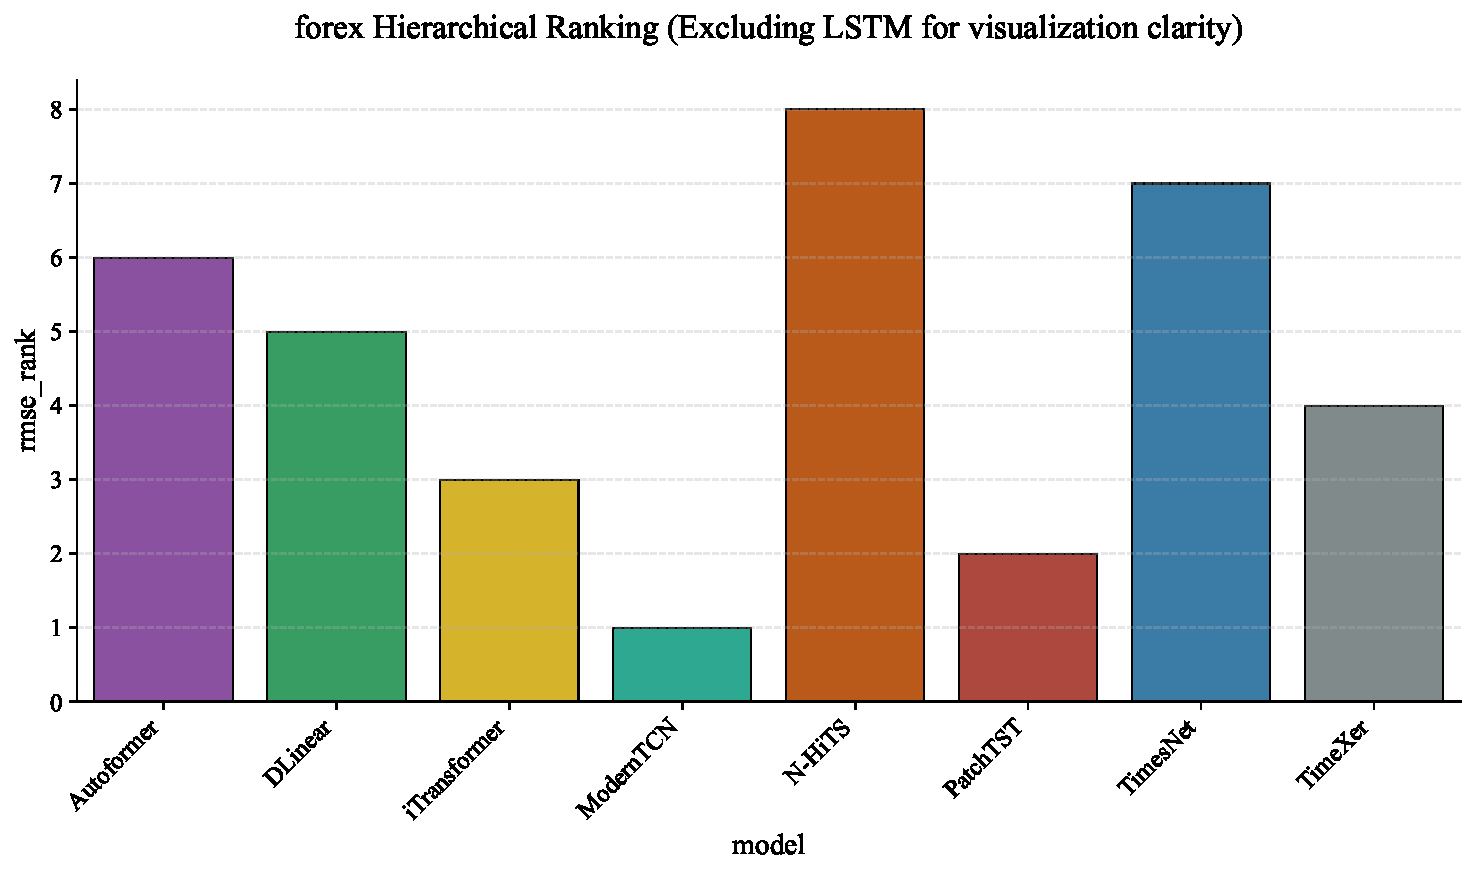
\includegraphics[width=\textwidth]{figures/04_category_analysis/forex_category_hierarchical_ranking_no_lstm.pdf}
    \caption{Forex.}
    \label{fig:app_forex_hier_ranking}
  \end{subfigure}
  \par\medskip
  \hfill
  \begin{subfigure}[b]{0.48\textwidth}
    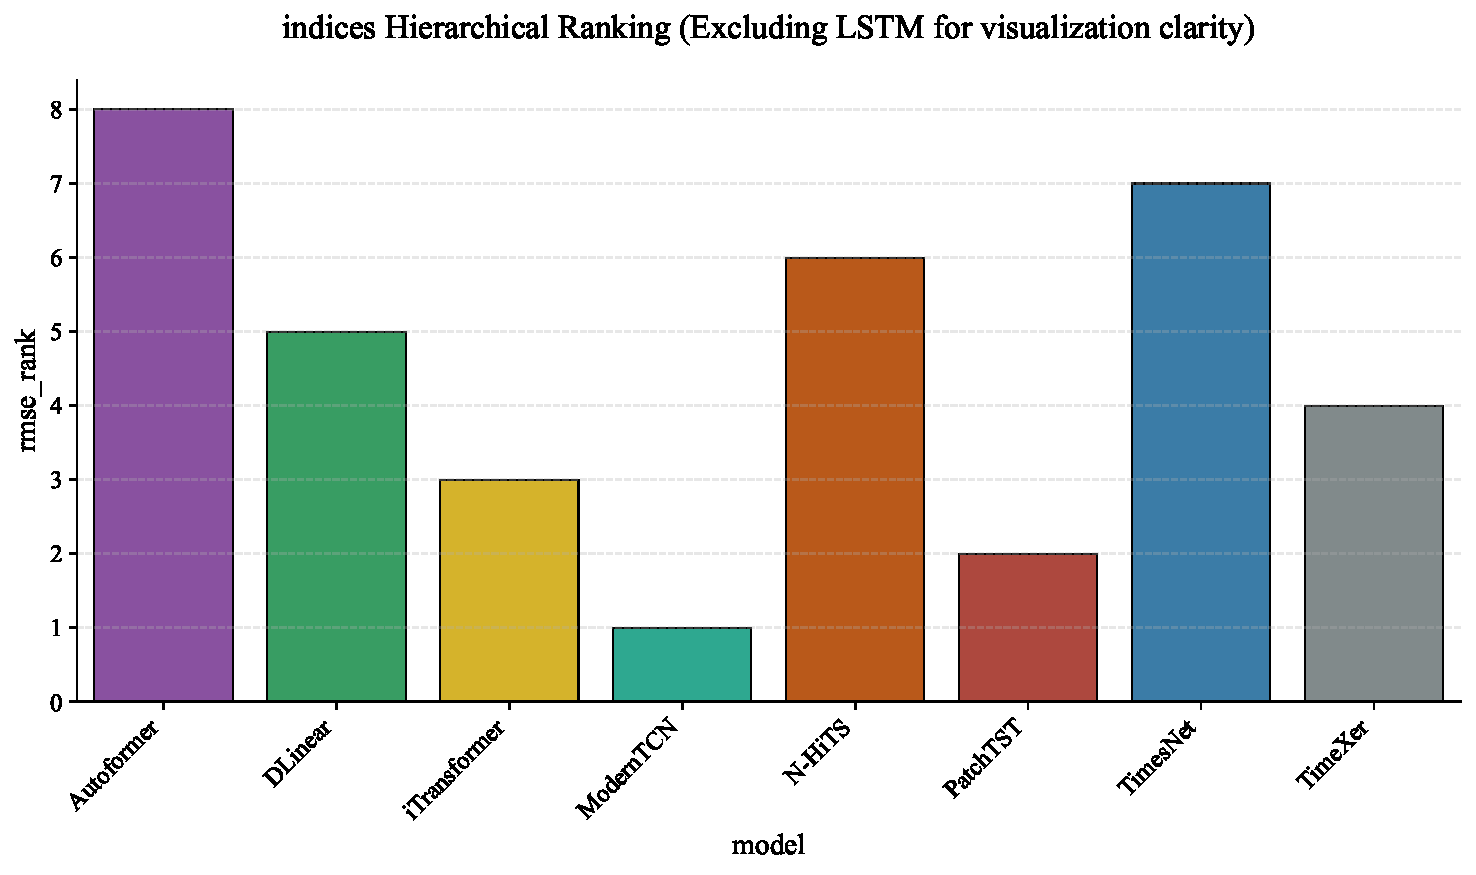
\includegraphics[width=\textwidth]{figures/04_category_analysis/indices_category_hierarchical_ranking_no_lstm.pdf}
    \caption{Equity Indices.}
    \label{fig:app_indices_hier_ranking}
  \end{subfigure}
  \hfill
  \caption{Category hierarchical ranking dendrograms for the eight modern architectures
           (\lstm excluded).  Branch lengths encode performance dissimilarity within
           each asset class.  \moderntcn and \patchtst are consistently co-clustered at
           the top of each dendrogram, confirming their joint dominance is stable
           across all three asset classes.}
  \label{fig:app_category_hierarchical_rankings}
\end{figure}

% --------------------------------------------------------------------------
\subsection{Category Performance Matrices}
\label{sec:app_category_matrices}

Figures~\ref{fig:app_crypto_perf_matrix}--\ref{fig:app_indices_perf_matrix} show
category performance matrices displaying normalised \rmse values for each model--asset
combination within each class, providing a complementary view to the overall leaderboard.
Rows represent models and columns represent assets; cell intensity encodes the normalised
error relative to the best model on that asset.

\begin{figure}[htbp]
  \centering
  \begin{subfigure}[b]{0.48\textwidth}
    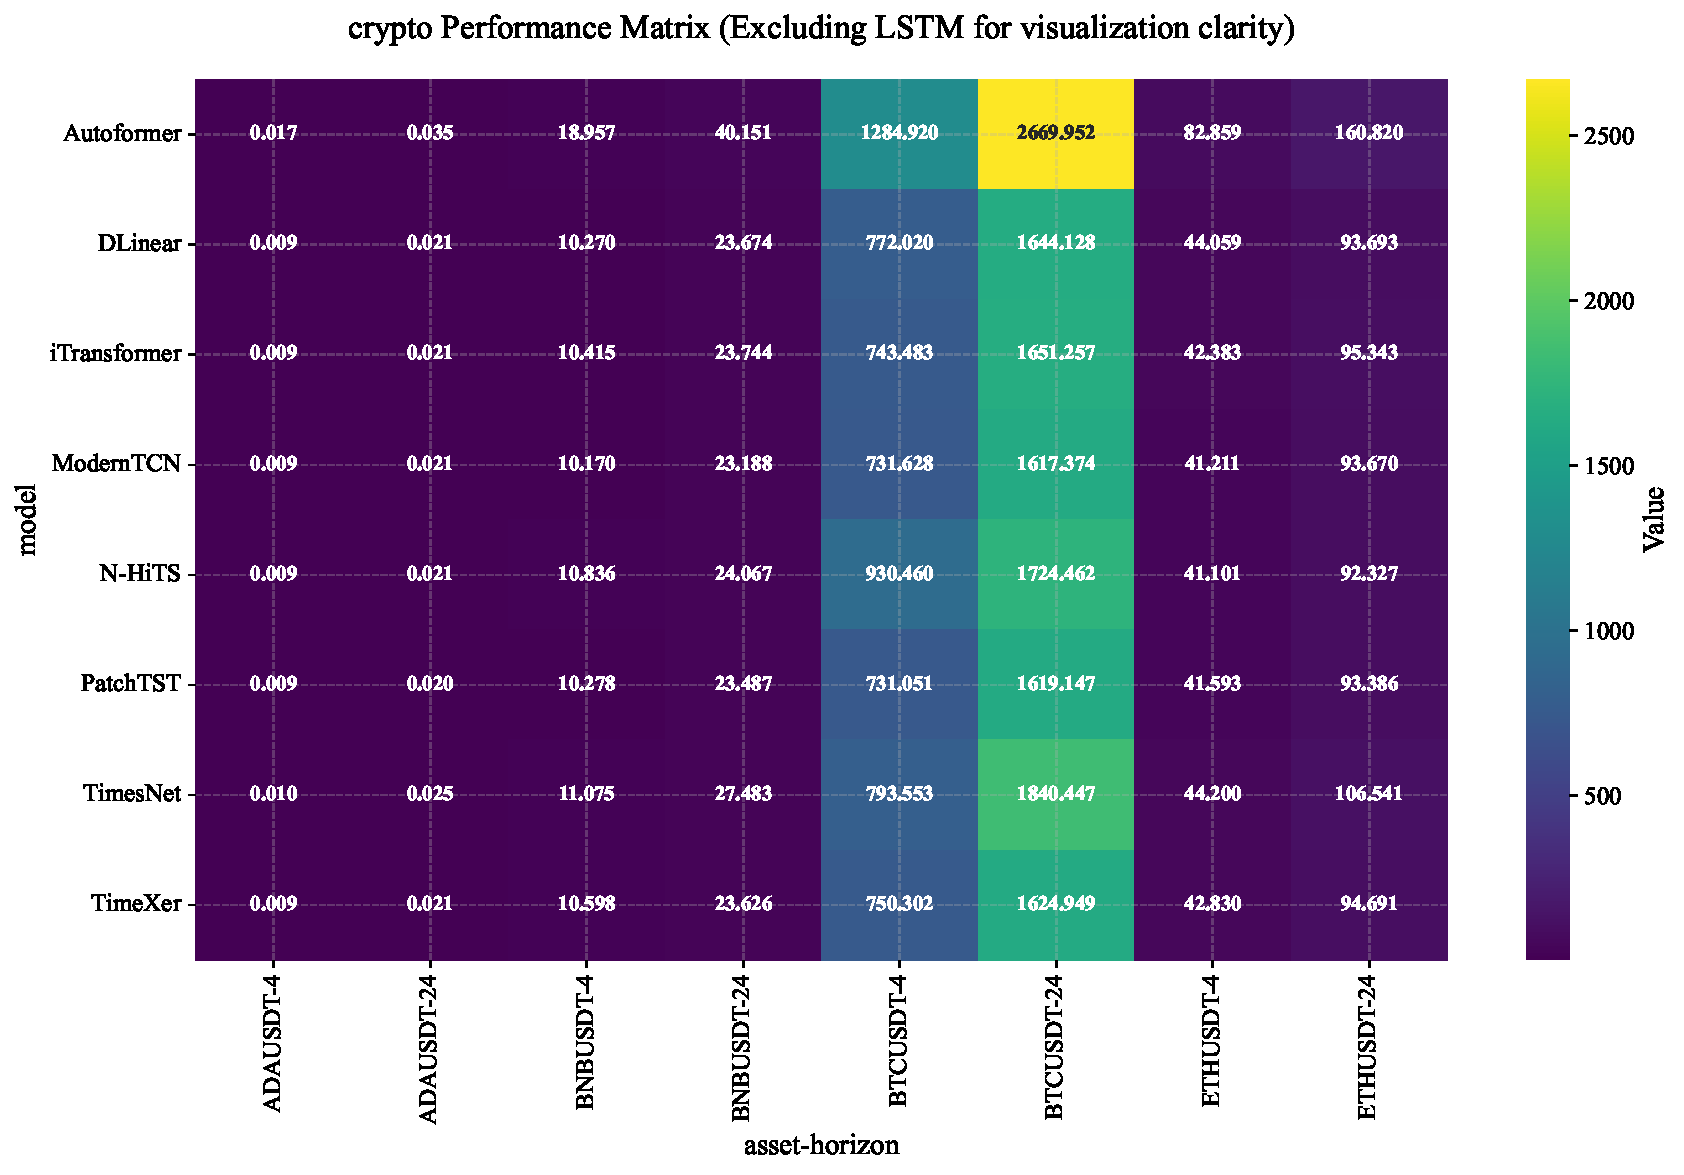
\includegraphics[width=\textwidth]{figures/04_category_analysis/crypto_category_performance_matrix_no_lstm.pdf}
    \caption{Cryptocurrency.}
    \label{fig:app_crypto_perf_matrix}
  \end{subfigure}
  \hfill
  \begin{subfigure}[b]{0.48\textwidth}
    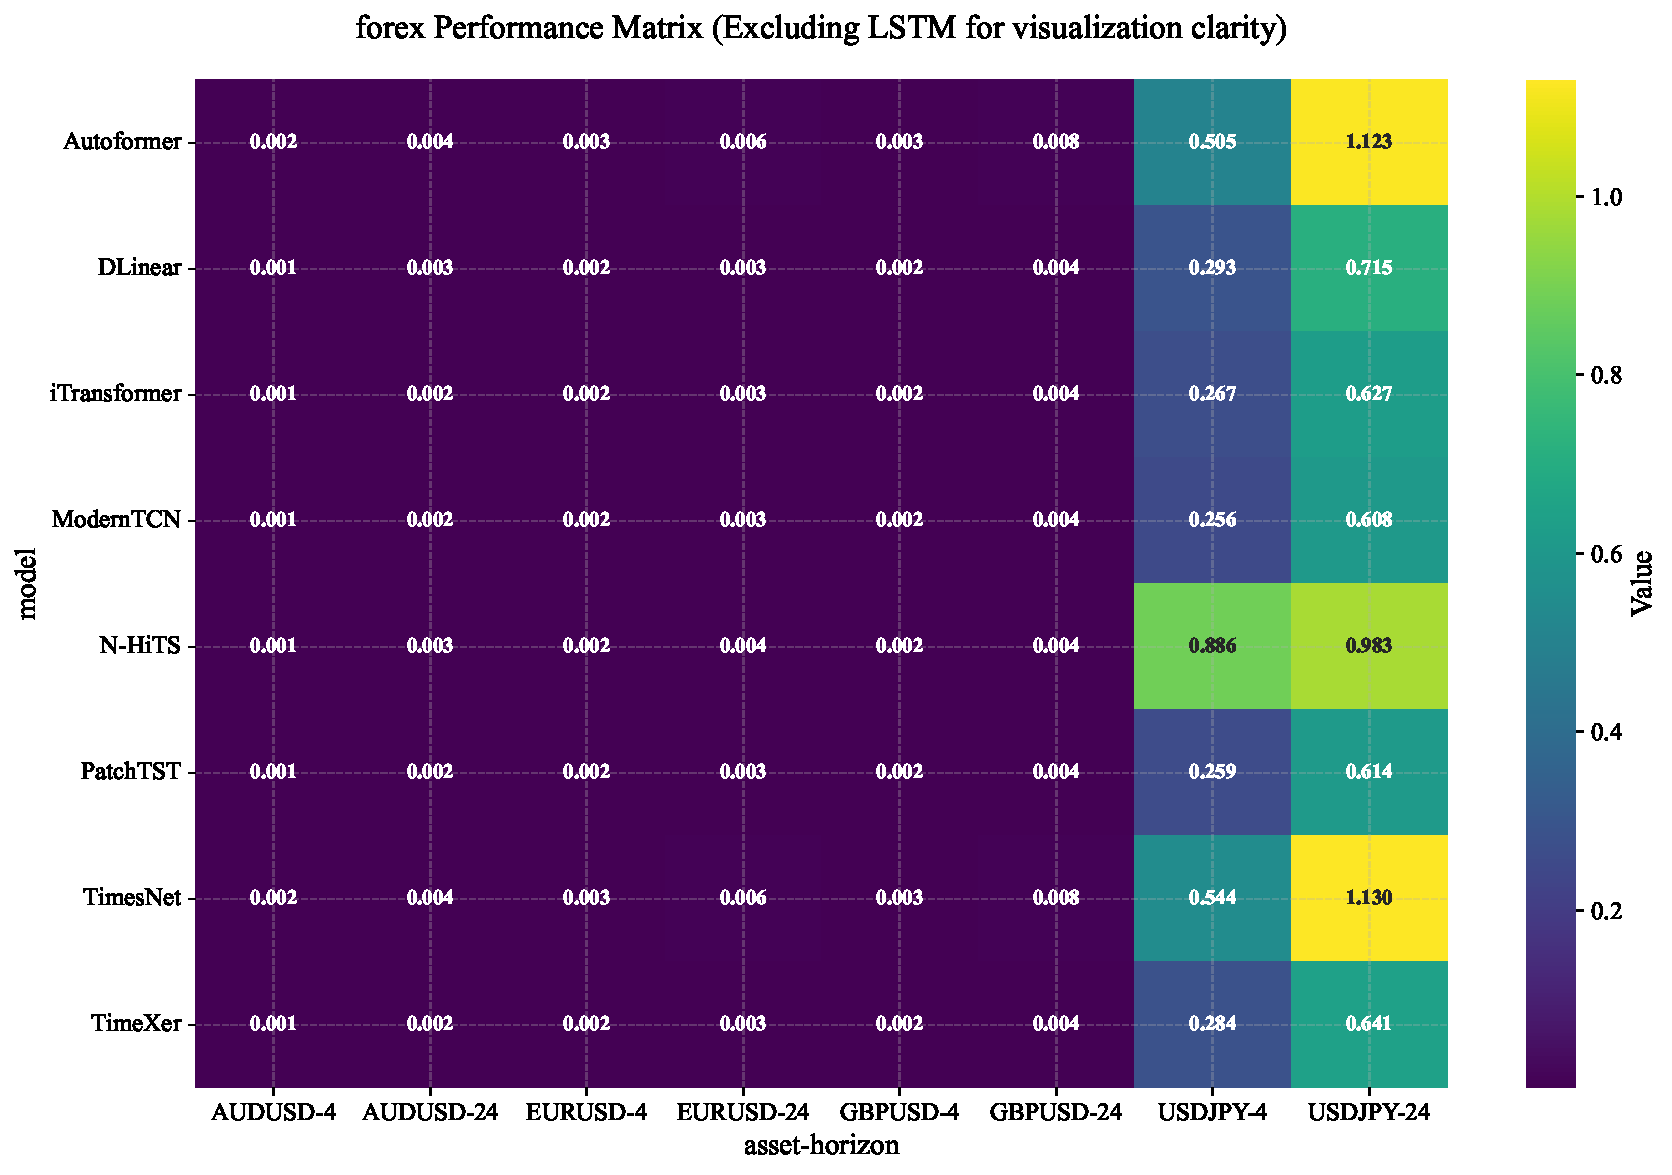
\includegraphics[width=\textwidth]{figures/04_category_analysis/forex_category_performance_matrix_no_lstm.pdf}
    \caption{Forex.}
    \label{fig:app_forex_perf_matrix}
  \end{subfigure}

  \par\medskip
  \centering
  \begin{subfigure}[b]{0.65\textwidth}
    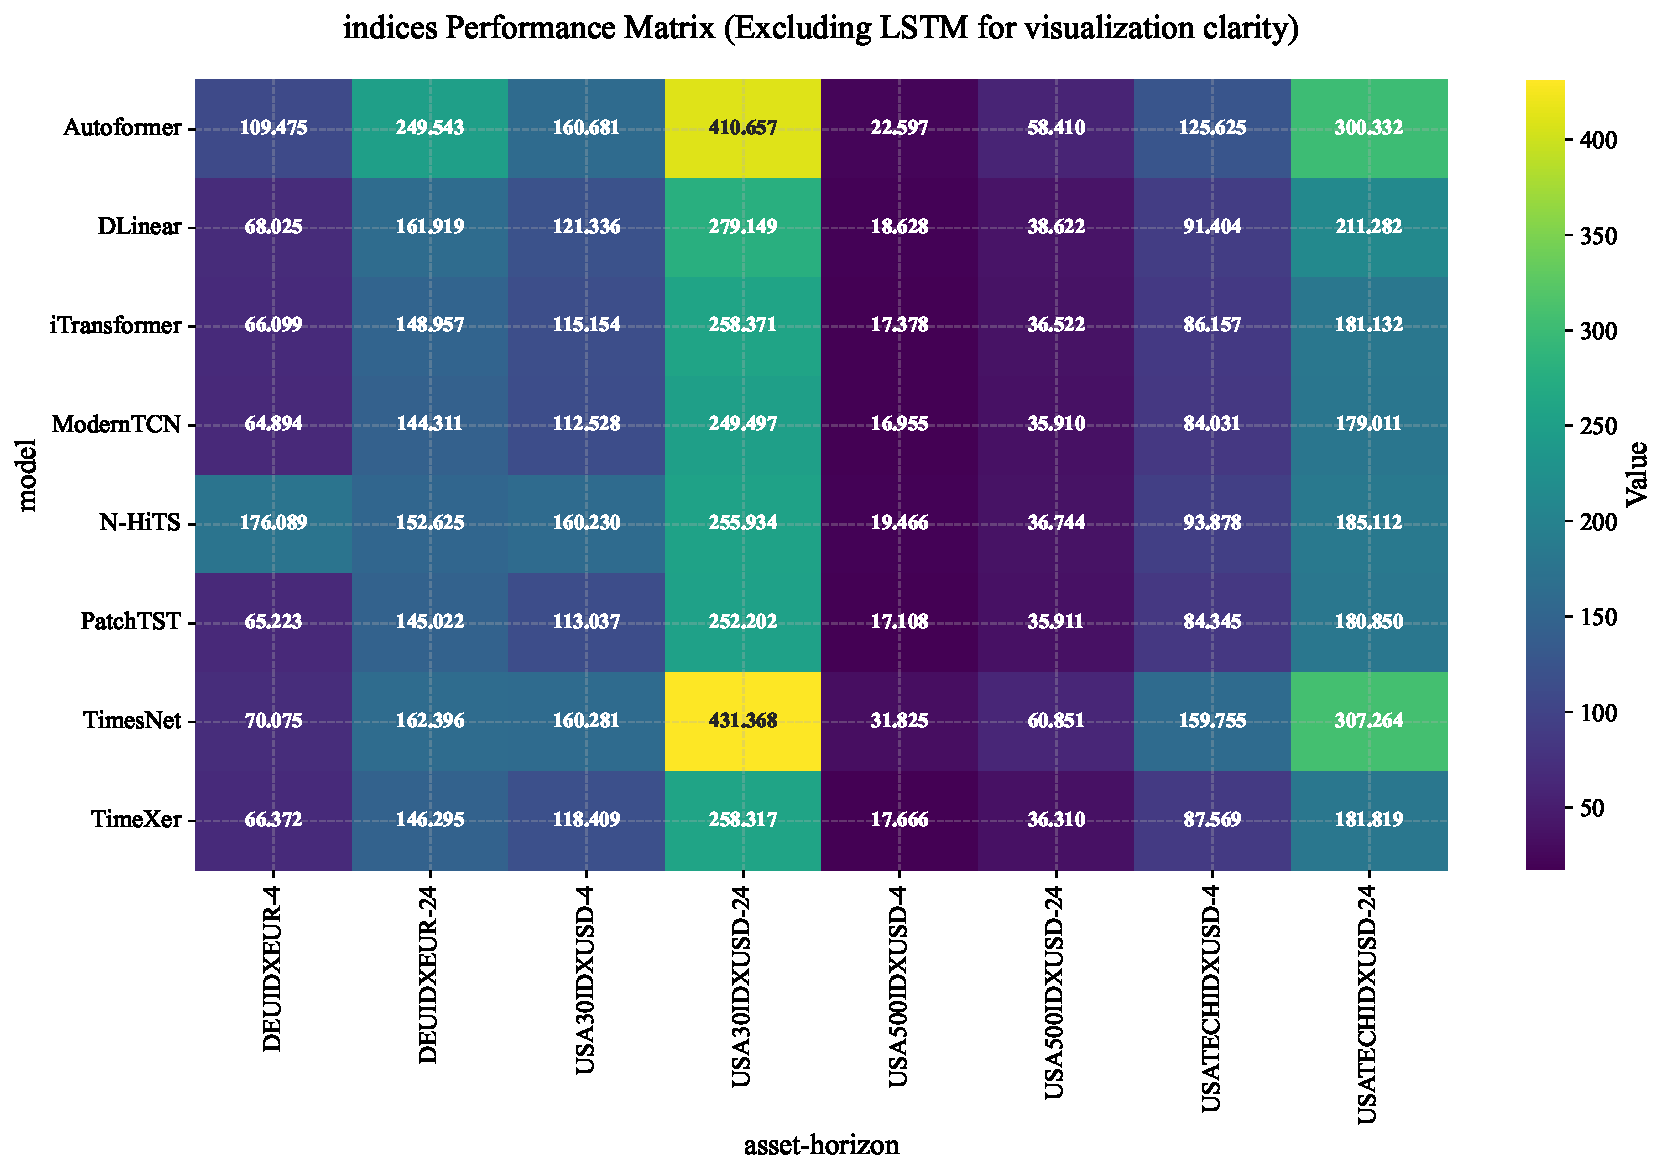
\includegraphics[width=\textwidth]{figures/04_category_analysis/indices_category_performance_matrix_no_lstm.pdf}
    \caption{Equity Indices.}
    \label{fig:app_indices_perf_matrix}
  \end{subfigure}

  \caption{Category performance matrices for the eight modern architectures (\lstm excluded).
           Cell intensity encodes normalised \rmse relative to the best model per asset
           (darker = worse).  \moderntcn and \patchtst occupy the lightest cells
           consistently; \autoformer and \timesnet occupy the darkest, confirming the
           three-tier structure observed in the global leaderboard.}
  \label{fig:app_category_performance_matrices}
\end{figure}

% =============================================================================
\section{Methodological Details}
\label{sec:app_methods}

% --------------------------------------------------------------------------
\subsection{Hyperparameter Search Spaces}
\label{sec:app_hpo_spaces}

Table~\ref{tab:hpo_search_spaces} in the main text summarises the HPO search dimensions for all
models.  The key varied parameters by model family are as follows.

\begin{itemize}[nosep]
  \item \textbf{Transformer models} (\autoformer, \patchtst, \itransformer, \timexer): model dimension,
        attention heads, encoder depth, feedforward width, dropout, learning rate, batch size, and
        architecture-specific parameters (patch configuration, moving-average windows).
  \item \textbf{MLP models} (\dlinear, \nhits): kernel size and decomposition mode (\dlinear); block
        count, hidden-layer width, depth, and pooling scales (\nhits).
  \item \textbf{CNN models} (\timesnet, \moderntcn): channel and depth parameters, dominant-frequency
        or patch-size settings, and model-specific design choices.
  \item \textbf{RNN model} (\lstm): hidden-state size, layer count, projection width, and
        directionality (unidirectional or bidirectional).
\end{itemize}

All shared training hyperparameters (learning-rate range, batch-size options) were held constant
across all models to ensure no implicit tuning advantage.  Complete YAML search-space definitions
for each model are available in the Online Supplementary Materials.

% --------------------------------------------------------------------------
\subsection{Training Protocol}
\label{sec:app_training}

Final models were trained across three random seeds (123, 456, 789) using the frozen
best-hyperparameter configurations identified during the HPO stage; no retuning was performed.
Checkpoints were saved at each epoch to support full resumability from the last completed epoch.
All randomness sources (\texttt{random}, NumPy, PyTorch CPU and CUDA) were seeded identically per
run, with \texttt{cudnn.deterministic=True} and \texttt{cudnn.benchmark=False} enforced throughout.
Note: \texttt{torch.use\_deterministic\_algorithms(True)} was \emph{not} enabled; minor
hardware-dependent floating-point variation is possible across GPU models (see
Section~\ref{sec:determinism}).  Full training logs are archived in the Online
Supplementary Materials.

% --------------------------------------------------------------------------
\subsection{Robustness Checks}
\label{sec:app_robustness}

Seed-variance box plots (Figures~\ref{fig:app_seed_boxplot_h4}--\ref{fig:app_seed_boxplot_h24})
and \rmse-versus-seed-variance scatter plots
(Figures~\ref{fig:app_scatter_seed_h4}--\ref{fig:app_scatter_seed_h24})
confirm that inter-seed variance is negligible relative to inter-model variance across
all asset classes and horizons.  Results for BTC/USDT, EUR/USD, and Dow Jones are shown;
remaining assets exhibit qualitatively identical patterns and are archived in the Online
Supplementary Materials.

\begin{figure}[htbp]
  \centering
  \begin{subfigure}[b]{0.48\textwidth}
    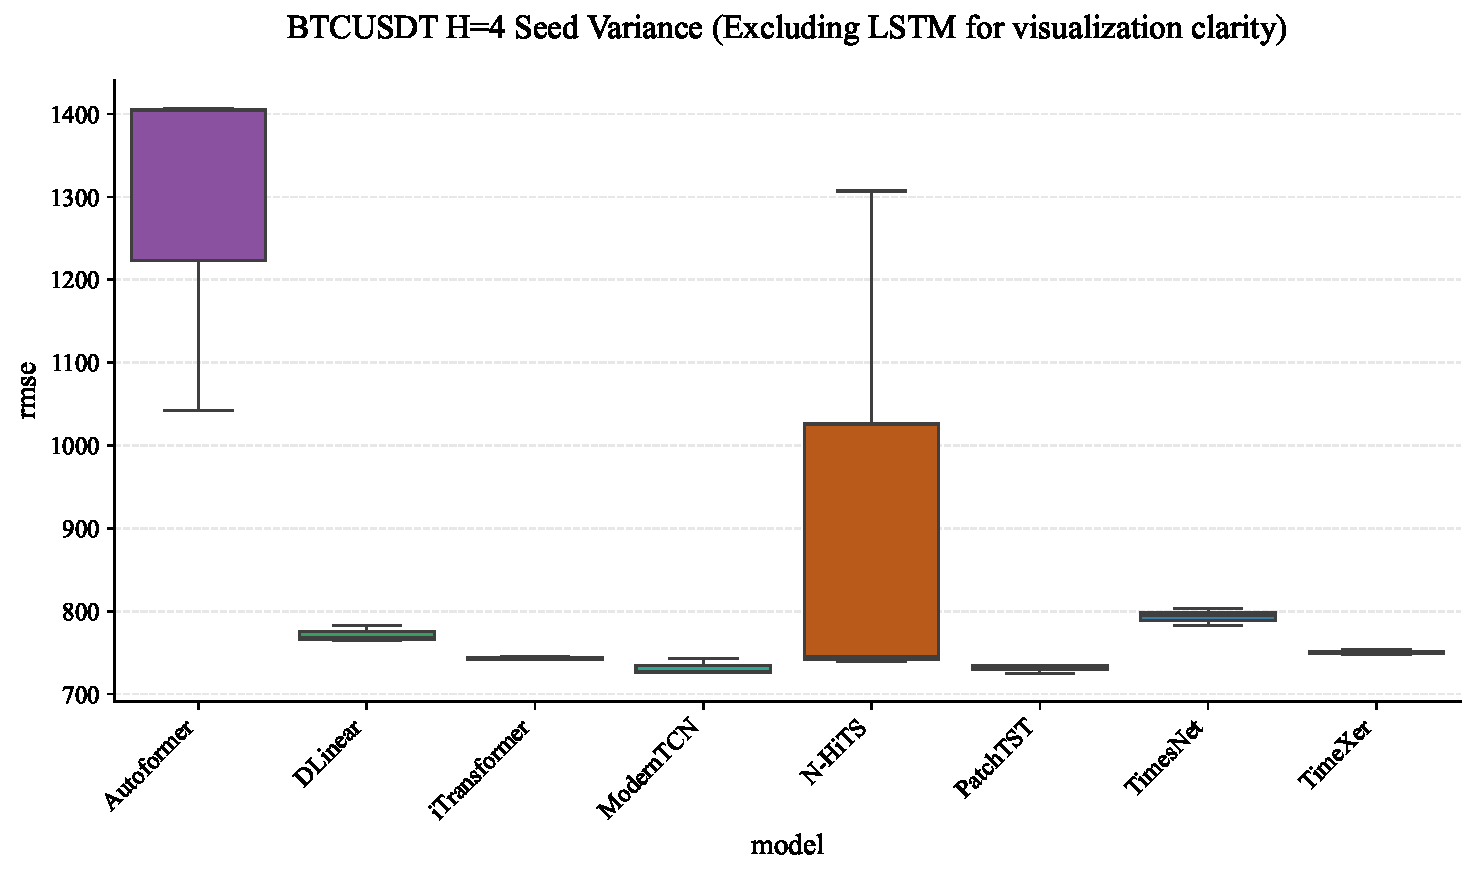
\includegraphics[width=\textwidth]{figures/06_robustness/btcusdt_h4_seed_variance_boxplot_no_lstm.pdf}
    \caption{BTC/USDT.}
    \label{fig:app_seed_boxplot_btc_h4}
  \end{subfigure}
  \hfill
  \begin{subfigure}[b]{0.48\textwidth}
    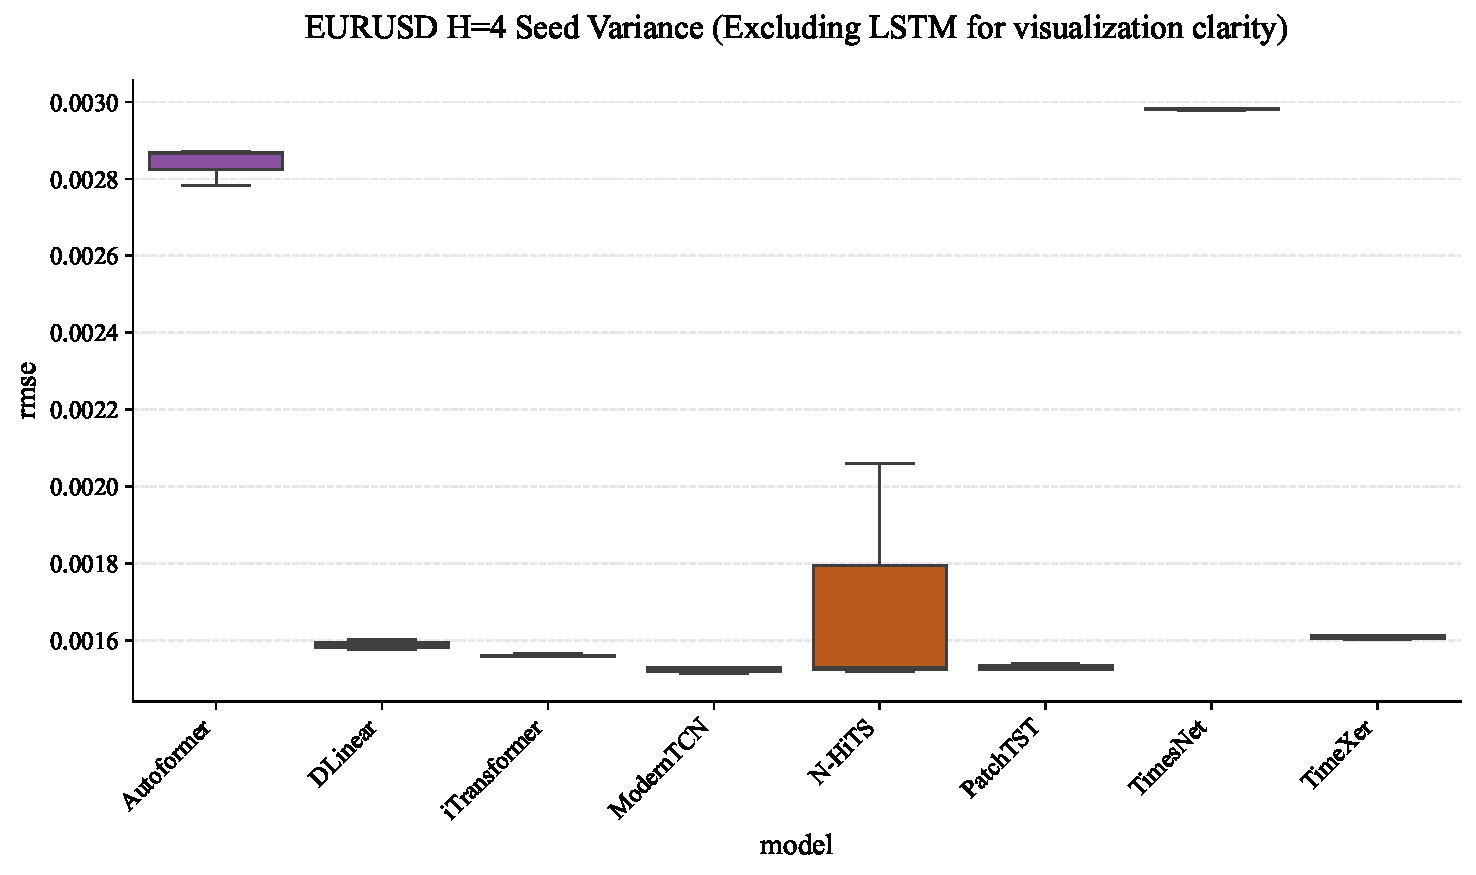
\includegraphics[width=\textwidth]{figures/06_robustness/eurusd_h4_seed_variance_boxplot_no_lstm.pdf}
    \caption{EUR/USD.}
    \label{fig:app_seed_boxplot_eur_h4}
  \end{subfigure}
  \par\medskip
  \centering
  \begin{subfigure}[b]{0.65\textwidth}
    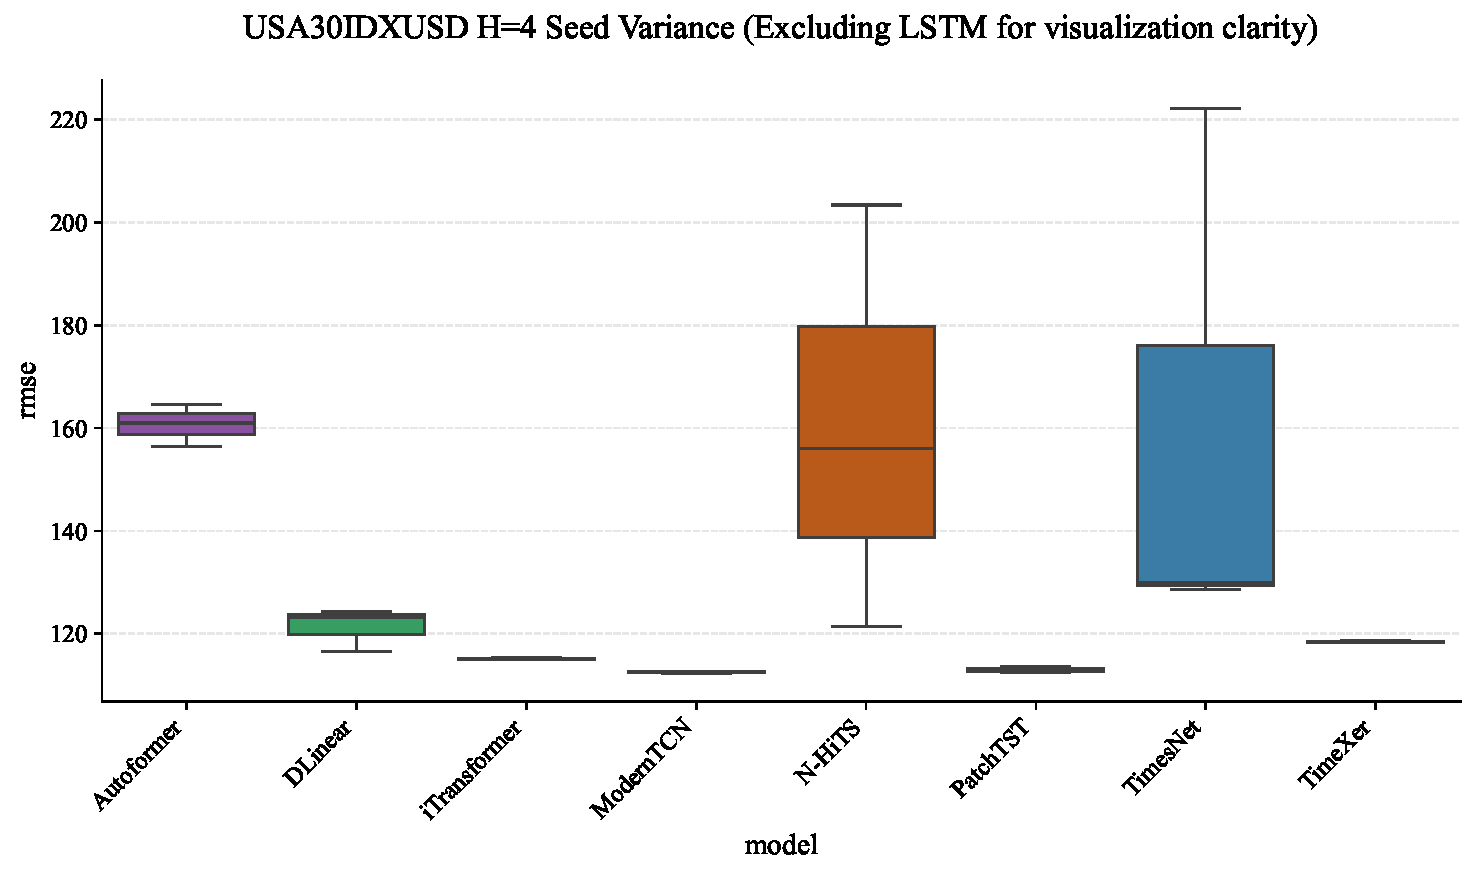
\includegraphics[width=\textwidth]{figures/06_robustness/usa30_h4_seed_variance_boxplot_no_lstm.pdf}
    \caption{Dow Jones.}
    \label{fig:app_seed_boxplot_usa30_h4}
  \end{subfigure}
  \caption{Seed-variance box plots at $\hfour$ for the three representative assets
           (\lstm excluded).  Each box spans the interquartile range of \rmse values
           across seeds~123, 456, and 789.  Negligible box widths relative to
           inter-model differences confirm that seed accounts for $< 0.1\%$ of total forecast variance.}
  \label{fig:app_seed_boxplot_h4}
\end{figure}

\begin{figure}[htbp]
  \centering
  \begin{subfigure}[b]{0.48\textwidth}
    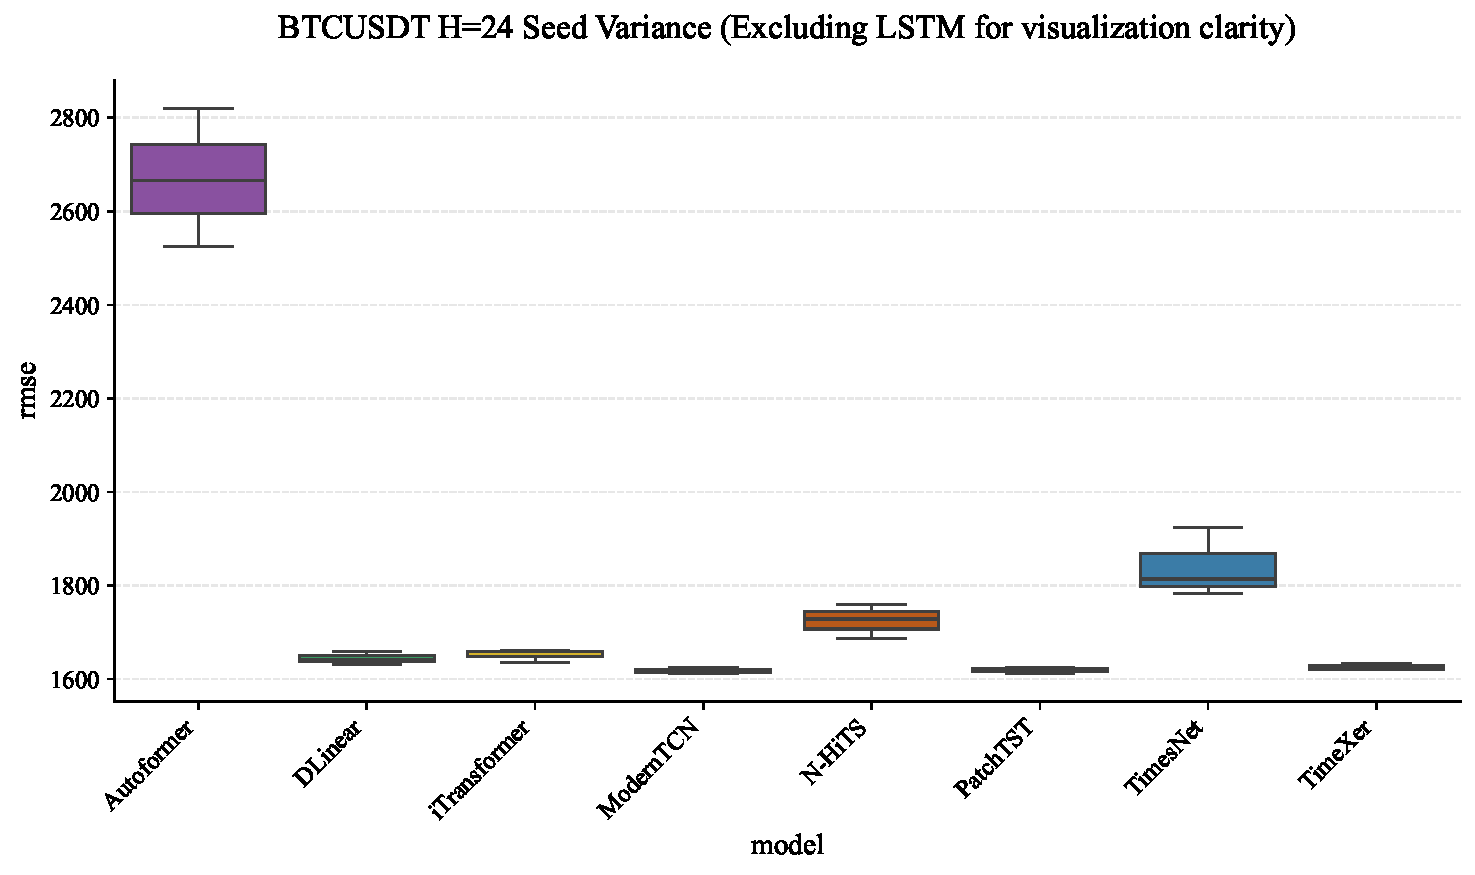
\includegraphics[width=\textwidth]{figures/06_robustness/btcusdt_h24_seed_variance_boxplot_no_lstm.pdf}
    \caption{BTC/USDT.}
    \label{fig:app_seed_boxplot_btc_h24}
  \end{subfigure}
  \hfill
  \begin{subfigure}[b]{0.48\textwidth}
    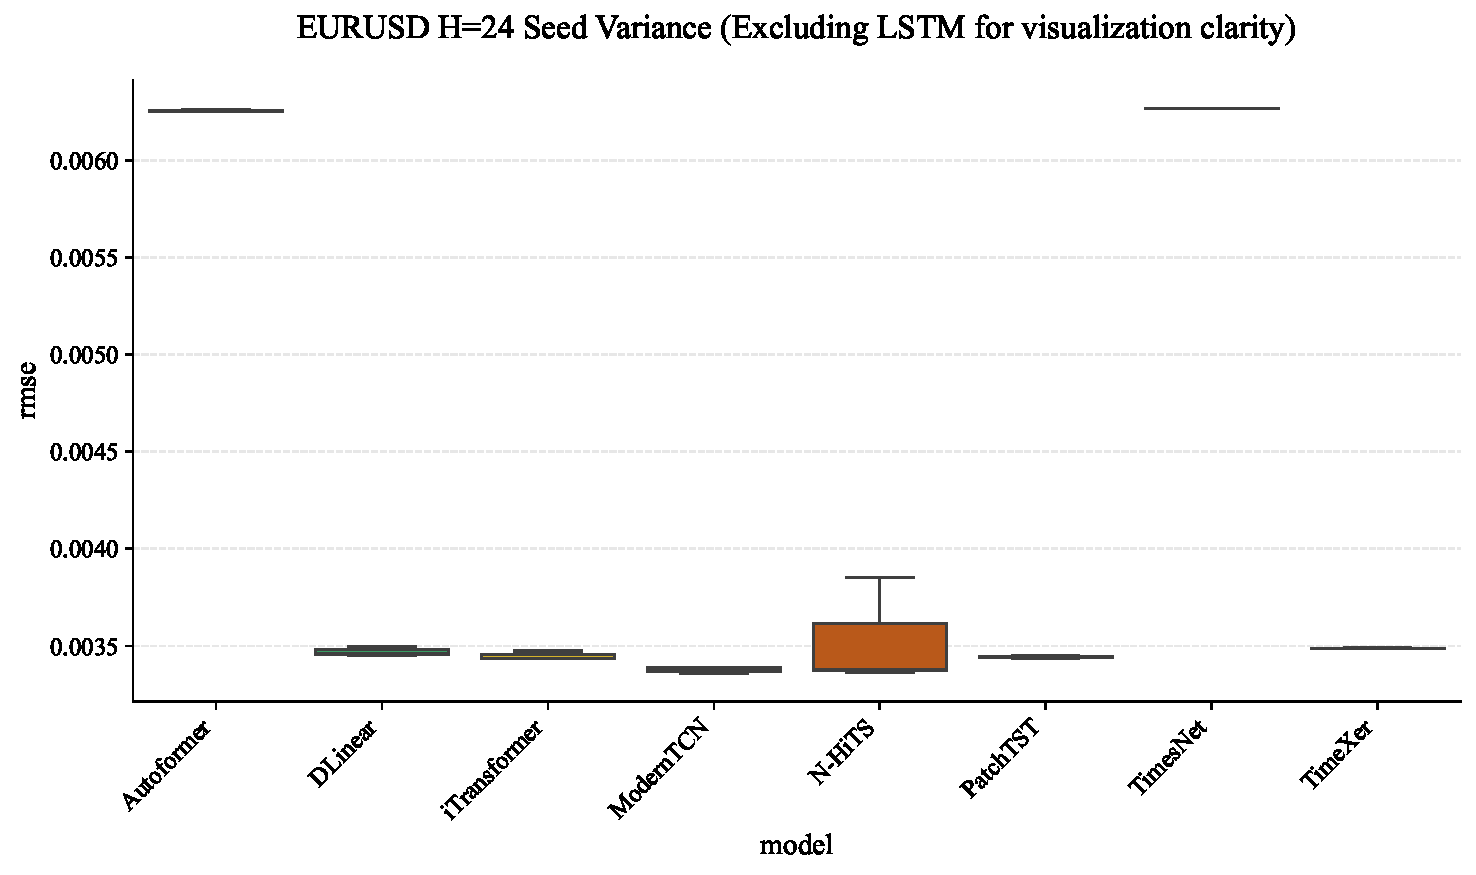
\includegraphics[width=\textwidth]{figures/06_robustness/eurusd_h24_seed_variance_boxplot_no_lstm.pdf}
    \caption{EUR/USD.}
    \label{fig:app_seed_boxplot_eur_h24}
  \end{subfigure}
  \par\medskip
  \centering
  \begin{subfigure}[b]{0.65\textwidth}
    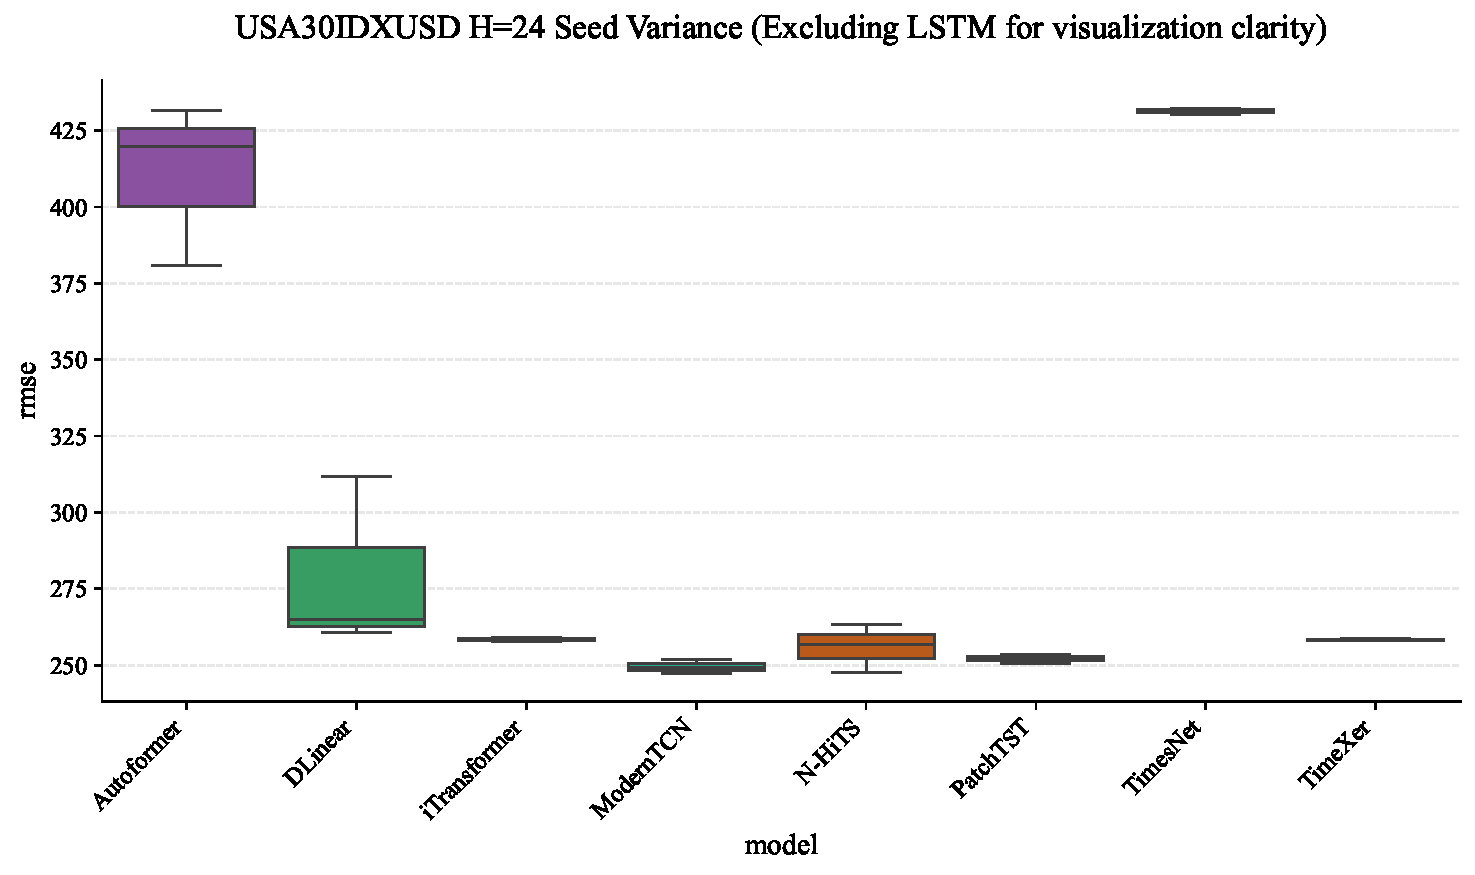
\includegraphics[width=\textwidth]{figures/06_robustness/usa30_h24_seed_variance_boxplot_no_lstm.pdf}
    \caption{Dow Jones.}
    \label{fig:app_seed_boxplot_usa30_h24}
  \end{subfigure}
  \caption{Seed-variance box plots at $\htwentyfour$ for the three representative assets
           (\lstm excluded).  The pattern mirrors $\hfour$: box widths remain negligible
           at the longer horizon, confirming H3 holds at both forecast depths.}
  \label{fig:app_seed_boxplot_h24}
\end{figure}

\begin{figure}[htbp]
  \centering
  \begin{subfigure}[b]{0.48\textwidth}
    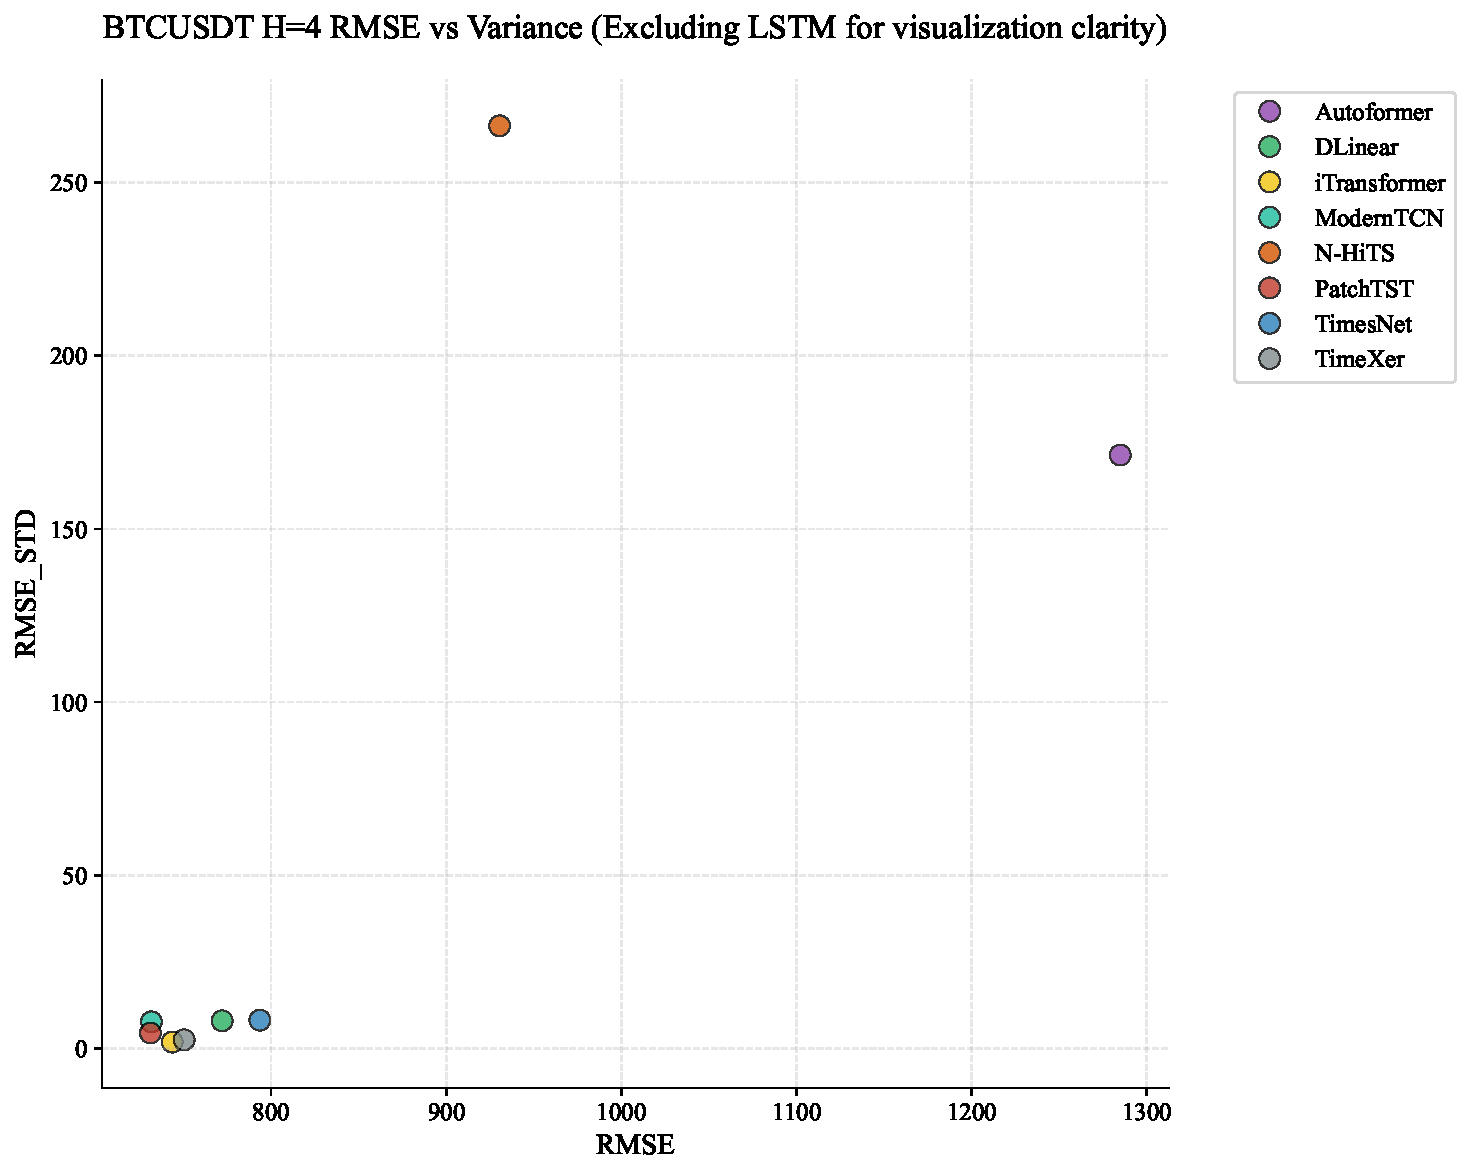
\includegraphics[width=\textwidth]{figures/06_robustness/btcusdt_h4_scatter_rmse_vs_seed_variance_no_lstm.pdf}
    \caption{BTC/USDT.}
    \label{fig:app_scatter_btc_h4}
  \end{subfigure}
  \hfill
  \begin{subfigure}[b]{0.48\textwidth}
    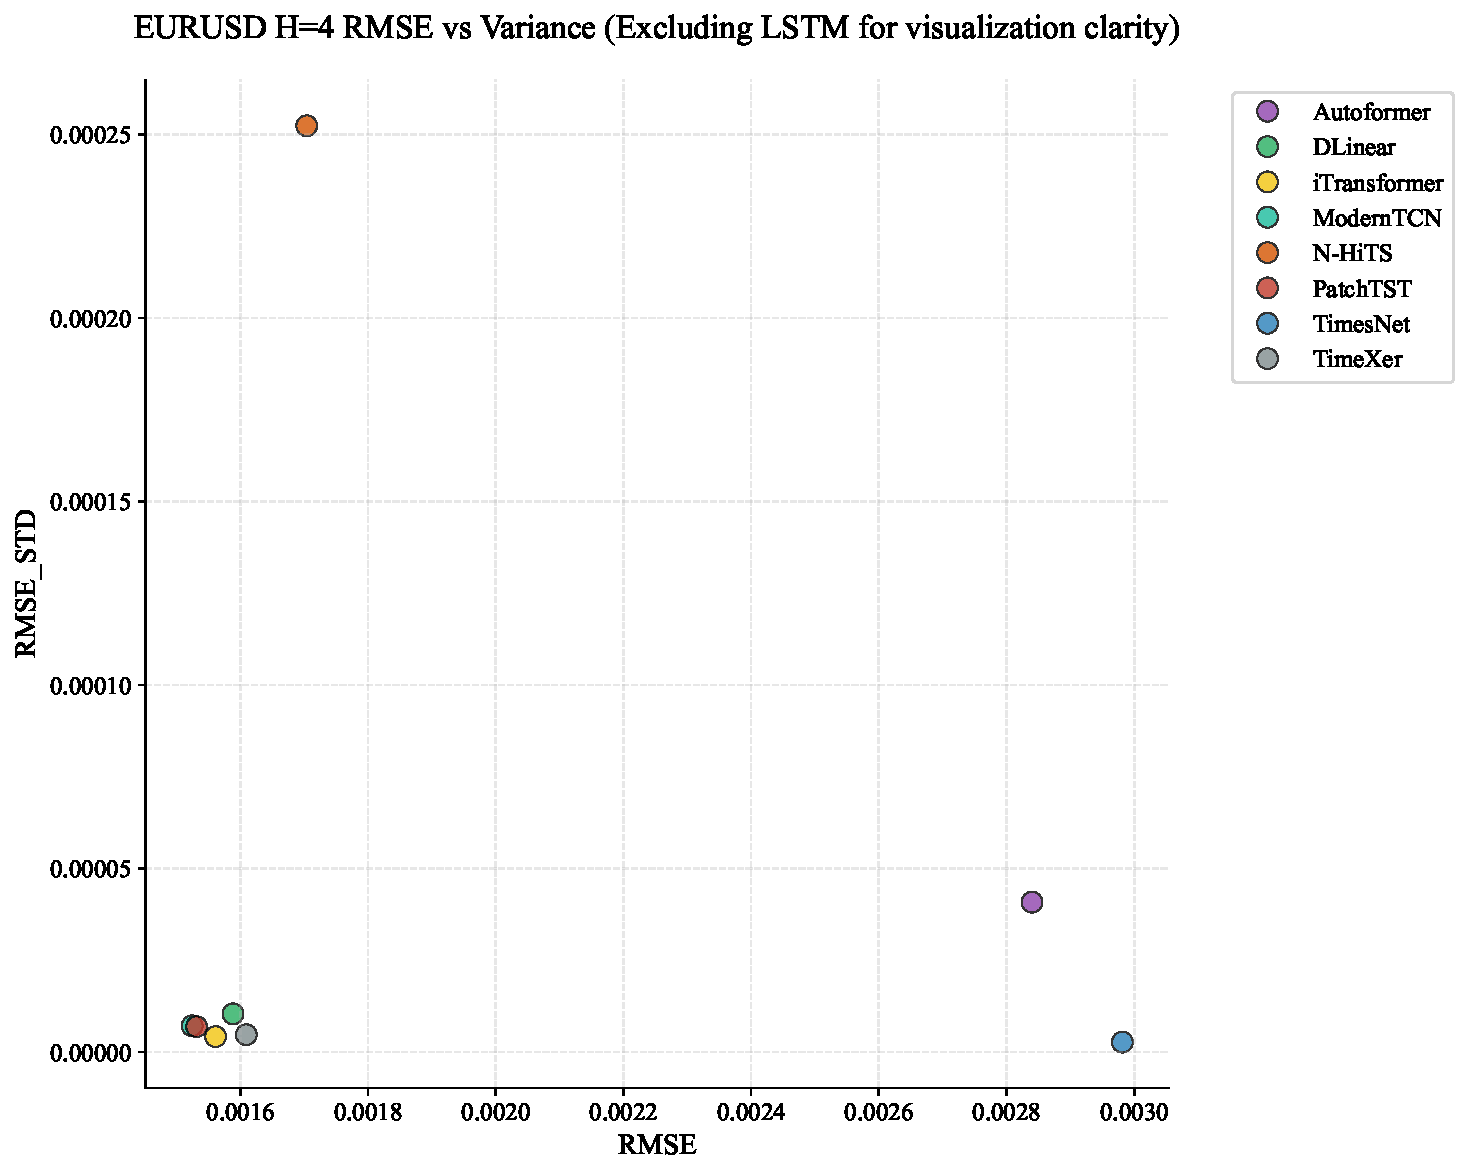
\includegraphics[width=\textwidth]{figures/06_robustness/eurusd_h4_scatter_rmse_vs_seed_variance_no_lstm.pdf}
    \caption{EUR/USD.}
    \label{fig:app_scatter_eur_h4}
  \end{subfigure}
  \par\medskip
  \centering
  \begin{subfigure}[b]{0.65\textwidth}
    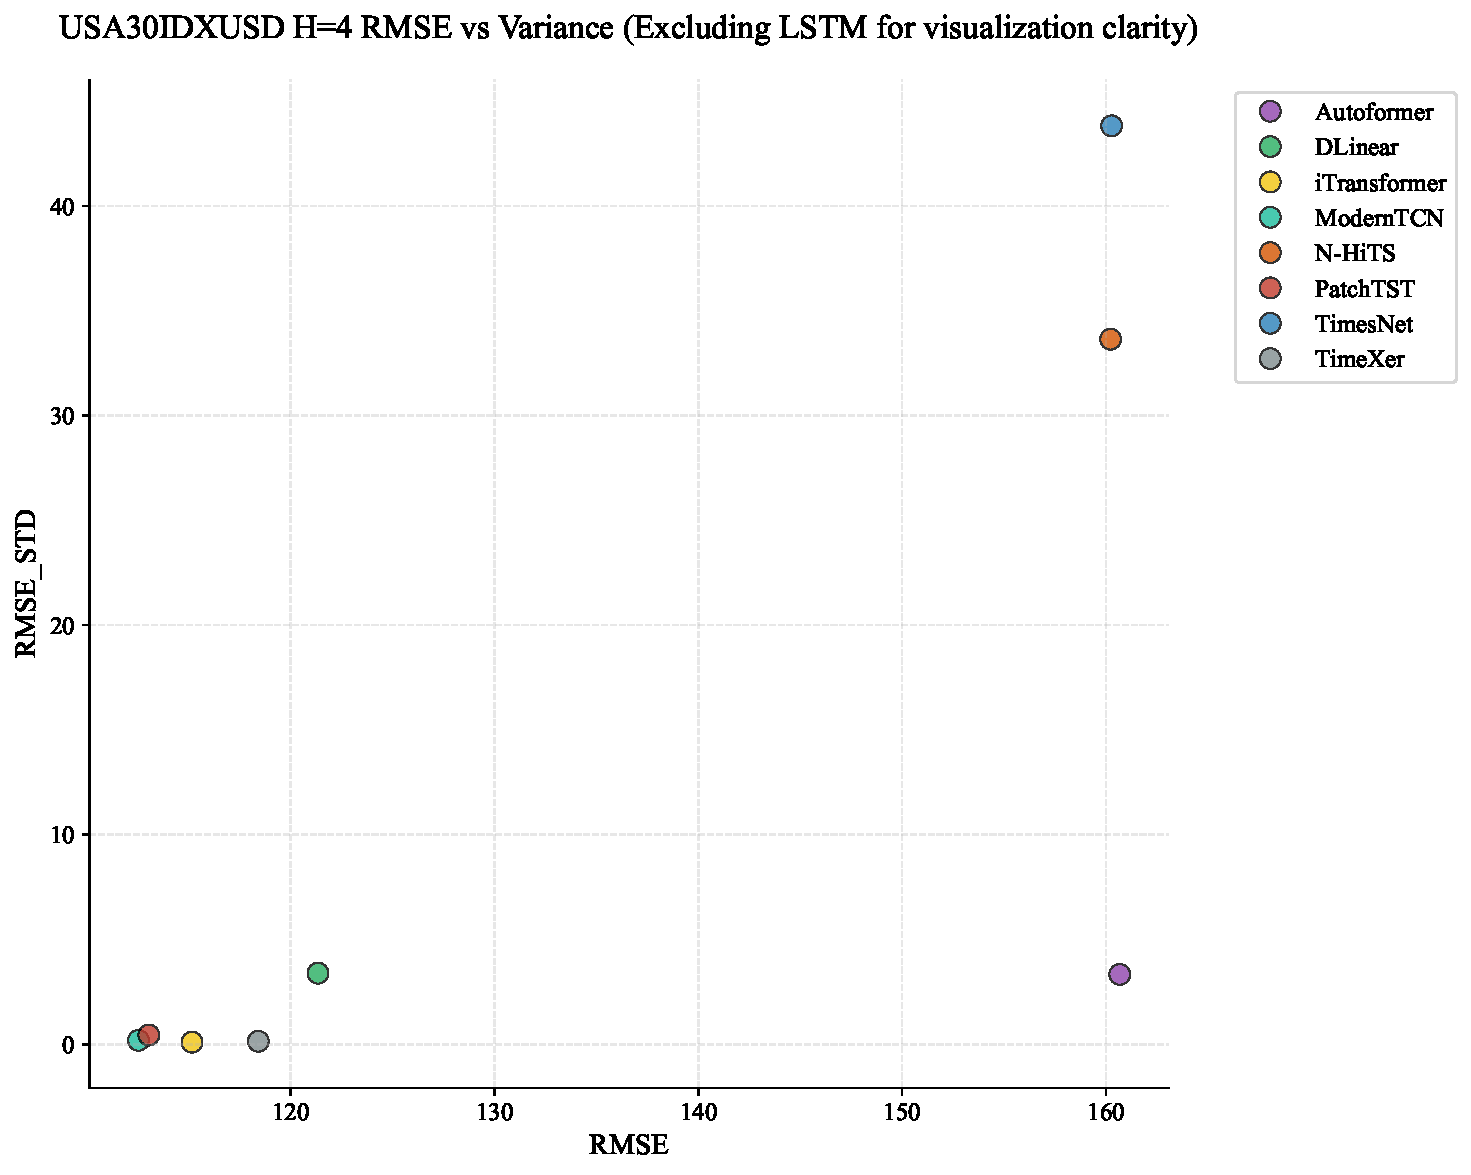
\includegraphics[width=\textwidth]{figures/06_robustness/usa30_h4_scatter_rmse_vs_seed_variance_no_lstm.pdf}
    \caption{Dow Jones.}
    \label{fig:app_scatter_usa30_h4}
  \end{subfigure}
  \caption{Mean \rmse vs.\ seed variance scatter at $\hfour$ for eight modern architectures.
           Each point represents one model; the horizontal axis shows mean \rmse across
           seeds, and the vertical axis shows the across-seed variance.  High-performing
           models (low mean \rmse) also exhibit low seed variance, confirming that
           architectural quality and robustness co-vary positively.}
  \label{fig:app_scatter_seed_h4}
\end{figure}

\begin{figure}[htbp]
  \centering
  \begin{subfigure}[b]{0.48\textwidth}
    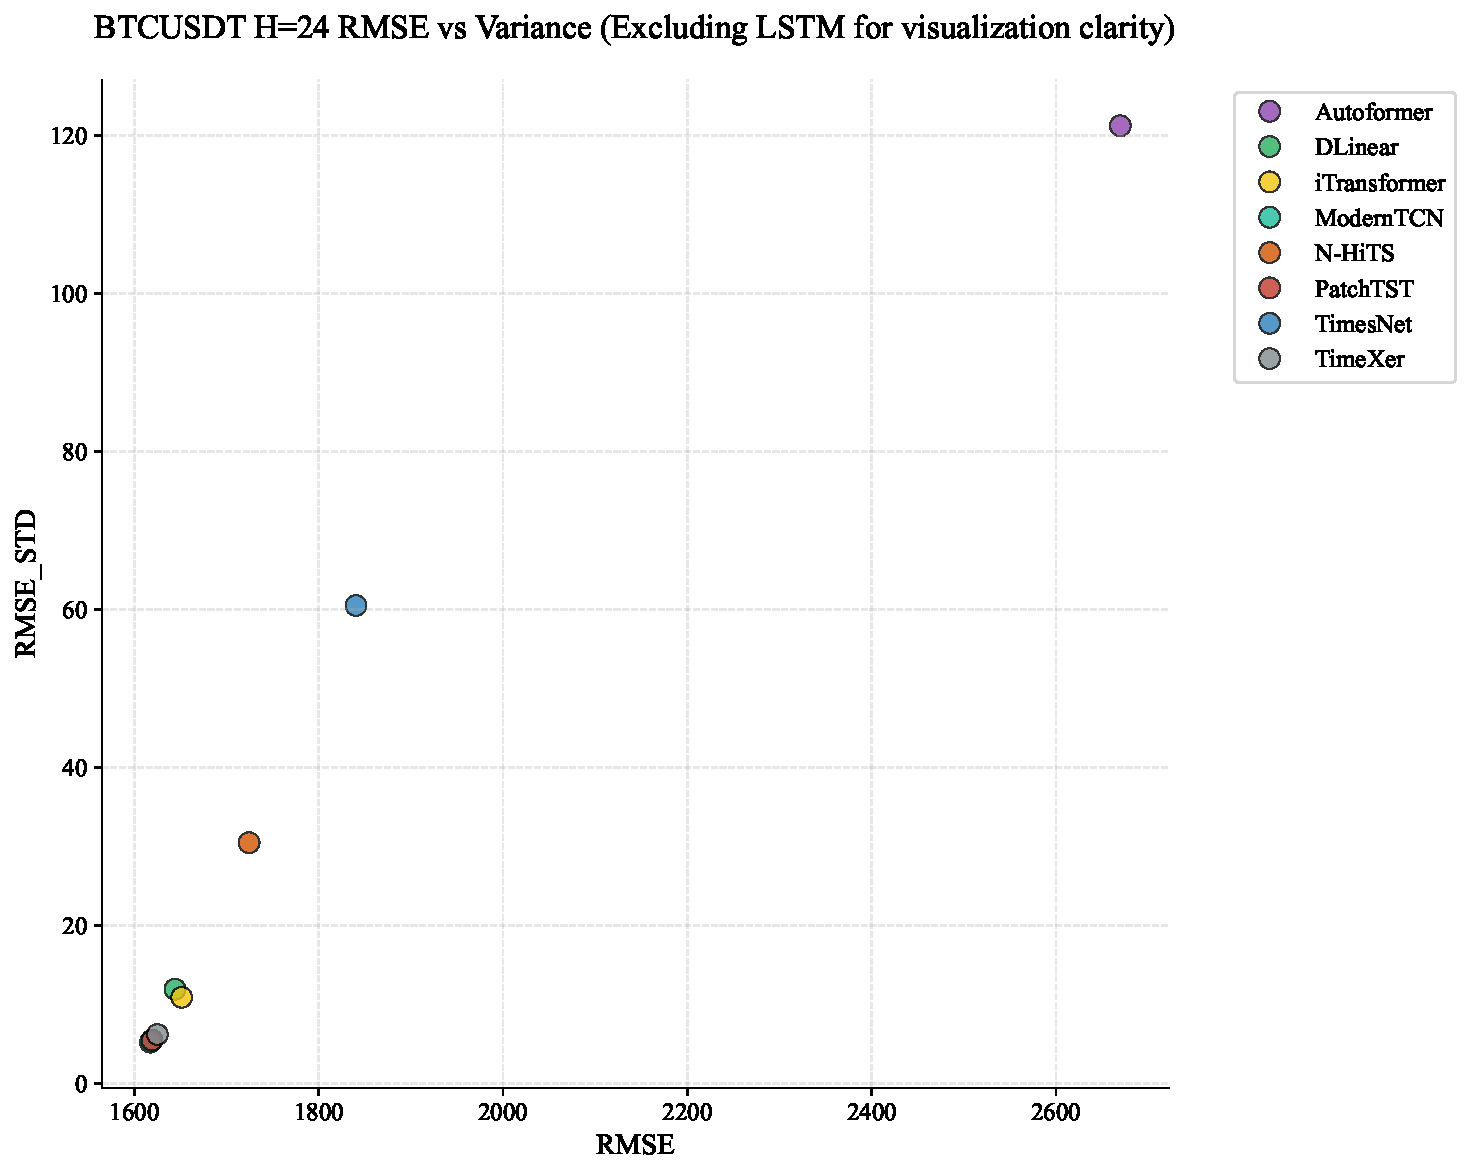
\includegraphics[width=\textwidth]{figures/06_robustness/btcusdt_h24_scatter_rmse_vs_seed_variance_no_lstm.pdf}
    \caption{BTC/USDT.}
    \label{fig:app_scatter_btc_h24}
  \end{subfigure}
  \hfill
  \begin{subfigure}[b]{0.48\textwidth}
    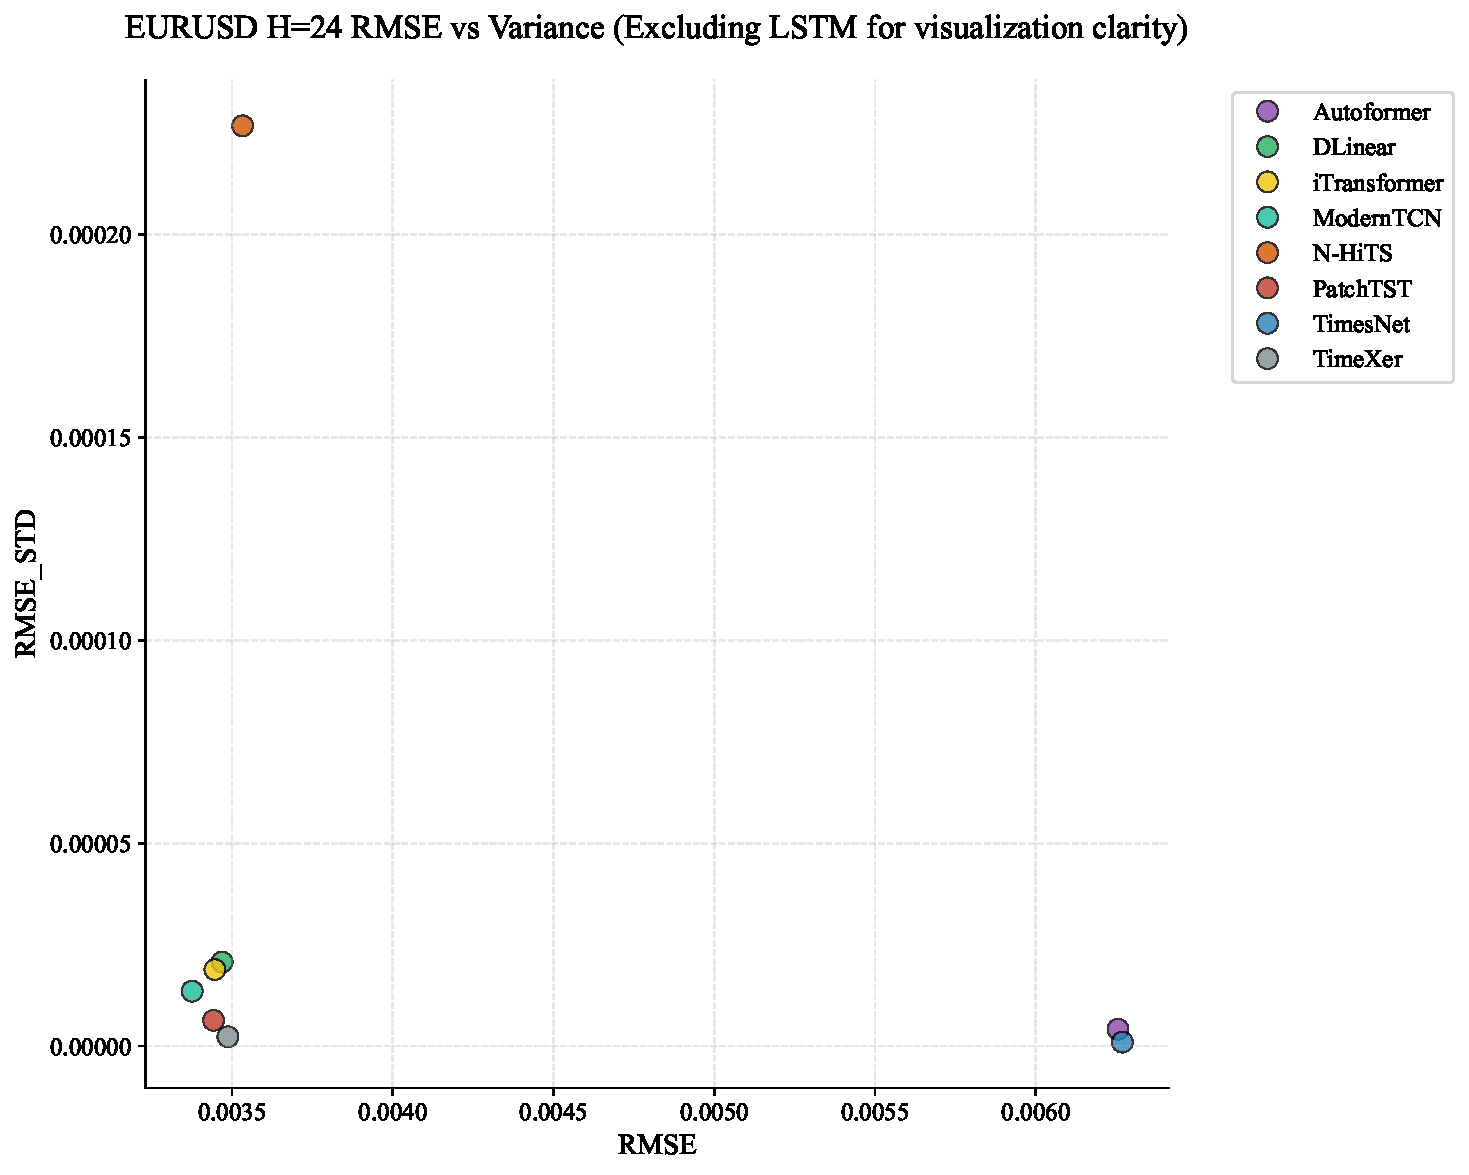
\includegraphics[width=\textwidth]{figures/06_robustness/eurusd_h24_scatter_rmse_vs_seed_variance_no_lstm.pdf}
    \caption{EUR/USD.}
    \label{fig:app_scatter_eur_h24}
  \end{subfigure}
  \par\medskip
  \centering
  \begin{subfigure}[b]{0.65\textwidth}
    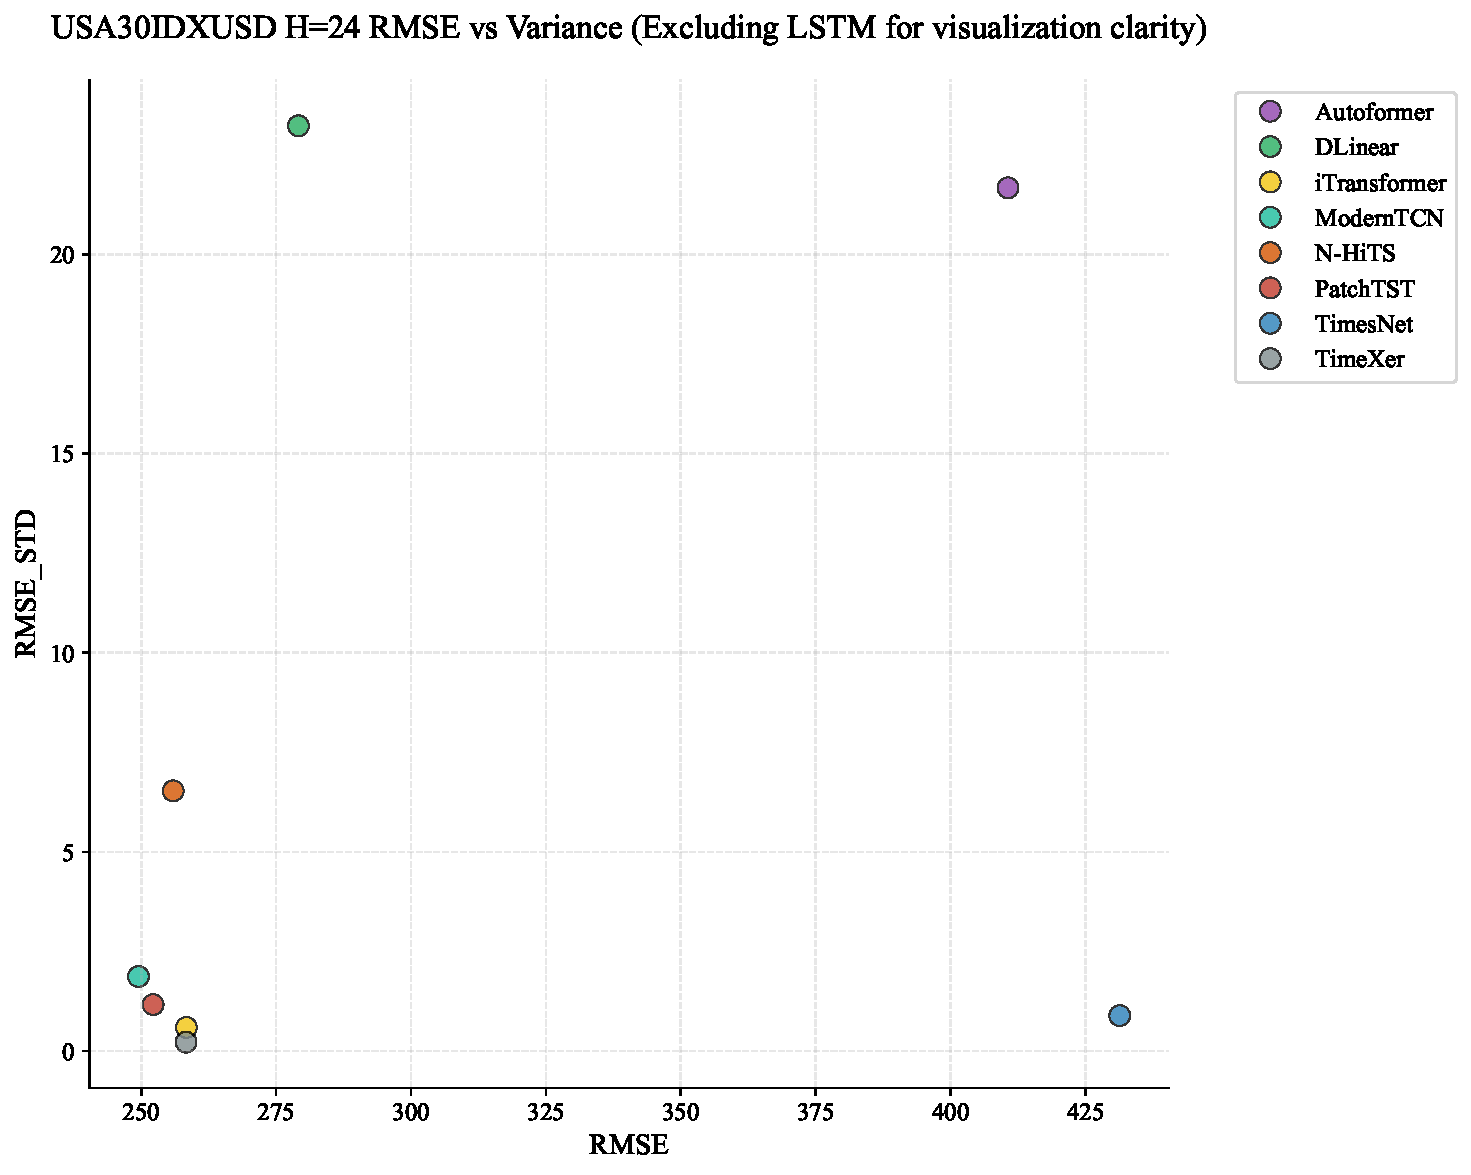
\includegraphics[width=\textwidth]{figures/06_robustness/usa30_h24_scatter_rmse_vs_seed_variance_no_lstm.pdf}
    \caption{Dow Jones.}
    \label{fig:app_scatter_usa30_h24}
  \end{subfigure}
  \caption{Mean \rmse vs.\ seed variance scatter at $\htwentyfour$.  The positive
           co-variation between performance and seed stability is maintained
           at the longer horizon.}
  \label{fig:app_scatter_seed_h24}
\end{figure}

% --------------------------------------------------------------------------
\subsection{Detailed Results and Figures}
\label{sec:app_repo}

While the main paper and this appendix present key empirical findings and summary visualisations, the full set of results from all 918 experimental runs is hosted in the project repository. This comprehensive archive ensures full transparency and supports independent verification of all reported metrics. The repository is available at:

\begin{center}
    \url{https://github.com/NabeelAhmad9/compare_forecasting_models}
\end{center}

The following content is available in the repository:
\begin{itemize}
    \item \textbf{Benchmark Results}: Complete \rmse, \mae, and \da scores for all 108 model--asset--horizon combinations across three seeds.
    \item \textbf{Figures}: High-resolution visualisations for all instruments, including per-seed actual vs.\ predicted plots.
    \item \textbf{Intermediate Outputs}: Full HPO trial logs, saved models and frozen best-hyperparameter configurations.
    \item \textbf{Training Artefacts}: All 648 trained model checkpoints and corresponding per-epoch CSV training logs.
    \item \textbf{Statistical Validation}: Raw outputs for all Friedman, \nem, and variance decomposition tests.
    \item \textbf{Full Project Code}: All scripts for models, training routines, benchmarking, evaluation, and utilities.
    \item \textbf{Notebooks}: Jupyter notebooks for running experiments, reproducing figures, and exploring intermediate results.
  \end{itemize}

% =============================================================================
\section*{Declaration of Interest}
\label{sec:declaration_of_interest}

The author declares that they have **no known competing financial interests or personal relationships** that could have influenced the research, analysis, or conclusions presented in this paper.